\documentclass[11pt,a4paper]{article}
% =====================================================================
% Informe de la Entrega 2 -- Grupo 6
% Estructura del informe final (sección 9 de la descripción del proyecto).
%
% Compilar:  latexmk -pdf Informe_Entrega2_Grupo6.tex   (o subir la carpeta a Overleaf)
% Dentro del repositorio usa ../../src/rsa_edu y ../../resultados/preliminar/figuras;
% fuera de él, las copias de las carpetas codigo/ y figuras/.
% Logo: colocar figuras/logo_unsaac.png (si no está, la portada se compila sin él).
% =====================================================================

% ------------------------------------------------------------------ paquetes
\usepackage[utf8]{inputenc}
\usepackage[T1]{fontenc}
\usepackage[spanish,provide=*]{babel}
\usepackage{mathptmx}
\usepackage[scaled=0.92]{helvet}
\usepackage{courier}
\usepackage{microtype}
\DisableLigatures[-]{encoding=T1,family=tt*} % que --metodo no se convierta en guion largo
\usepackage[a4paper,margin=2.5cm]{geometry}
\usepackage{amsmath,amssymb}
\usepackage{graphicx}
\usepackage{xcolor}
\usepackage{booktabs,tabularx,multirow,array,longtable,makecell}
\usepackage{enumitem}
\usepackage{float}
\usepackage{caption,subcaption}
\usepackage{algorithm}
\usepackage[noend]{algpseudocode}
\usepackage{listings}
\usepackage{tikz}
\usetikzlibrary{positioning,arrows.meta,shapes.geometric,fit,backgrounds,calc}
\usepackage{fancyhdr}
\usepackage{needspace}
\usepackage[most]{tcolorbox}
\usepackage[hidelinks]{hyperref}
\urlstyle{same}

\definecolor{azul}{HTML}{2A78D6}
\definecolor{naranja}{HTML}{EB6834}
\definecolor{verde}{HTML}{1BAF7A}
\definecolor{gris}{HTML}{52514E}
\definecolor{fondo}{HTML}{F6F6F4}
\definecolor{grisclaro}{HTML}{E4E3DF}

\captionsetup{font=small,labelfont=bf}
\setlist{nosep,leftmargin=*}
\renewcommand{\arraystretch}{1.15}
\newcolumntype{Y}{>{\raggedright\arraybackslash}X}
\newcolumntype{R}[1]{>{\raggedright\arraybackslash}p{#1}}
\setlength{\emergencystretch}{3em}
% Permitir cortes de línea después de los guiones bajos de nombres de archivos y funciones.
\let\guionbajo\_
\renewcommand{\_}{\guionbajo\allowbreak}

\newcommand{\estado}[1]{\textsf{\small[#1]}}

% ------------------------------------------------------------------ pseudocódigo en español
\floatname{algorithm}{Algoritmo}
\algrenewcommand\algorithmicrequire{\textbf{Entrada:}}
\algrenewcommand\algorithmicensure{\textbf{Salida:}}
\algrenewcommand\algorithmicwhile{\textbf{mientras}}
\algrenewcommand\algorithmicdo{\textbf{hacer}}
\algrenewcommand\algorithmicfor{\textbf{para}}
\algrenewcommand\algorithmicforall{\textbf{para cada}}
\algrenewcommand\algorithmicif{\textbf{si}}
\algrenewcommand\algorithmicthen{\textbf{entonces}}
\algrenewcommand\algorithmicelse{\textbf{si no}}
\algrenewcommand\algorithmicreturn{\textbf{devolver}}
\algrenewcommand\algorithmicfunction{\textbf{función}}
\algrenewcommand\algorithmicrepeat{\textbf{repetir}}
\algrenewcommand\algorithmicuntil{\textbf{hasta que}}
\algnewcommand\Break{\textbf{salir del bucle}}
\algnewcommand\Continue{\textbf{continuar}}
\algnewcommand\Error[1]{\textbf{error}(\textit{#1})}
\algrenewcommand\alglinenumber[1]{\scriptsize #1:}
\newcommand{\Mod}{\bmod}

% ------------------------------------------------------------------ código y salidas
\lstdefinestyle{py}{
  language=Python,
  basicstyle=\ttfamily\scriptsize,
  keywordstyle=\color{azul}\bfseries,
  commentstyle=\color{gris}\itshape,
  stringstyle=\color{naranja!80!black},
  numbers=left, numberstyle=\tiny\color{gris}, numbersep=6pt,
  backgroundcolor=\color{fondo}, frame=single, rulecolor=\color{grisclaro},
  xleftmargin=2.2em, framexleftmargin=1.8em,
  breaklines=true, breakatwhitespace=true, showstringspaces=false,
  columns=fullflexible, keepspaces=true, tabsize=4,
  extendedchars=true, inputencoding=utf8,
  literate={á}{{\'a}}1 {é}{{\'e}}1 {í}{{\'i}}1 {ó}{{\'o}}1 {ú}{{\'u}}1
           {ñ}{{\~n}}1 {Á}{{\'A}}1 {É}{{\'E}}1 {Ó}{{\'O}}1 {Ñ}{{\~N}}1
           {–}{{--}}1 {≤}{{$\le$}}1 {·}{{$\cdot$}}1 {×}{{$\times$}}1
           {¿}{{?`}}1 {¡}{{!`}}1 {ü}{{\"u}}1 {Í}{{\'I}}1 {Ú}{{\'U}}1
}
\lstdefinestyle{datos}{
  language={}, numbers=none, basicstyle=\ttfamily\scriptsize, backgroundcolor=\color{fondo},
  frame=single, rulecolor=\color{grisclaro}, columns=fullflexible,
  keepspaces=true, breaklines=false, showstringspaces=false,
  extendedchars=true, inputencoding=utf8,
  literate={á}{{\'a}}1 {é}{{\'e}}1 {í}{{\'i}}1 {ó}{{\'o}}1 {ú}{{\'u}}1 {ñ}{{\~n}}1
           {Á}{{\'A}}1 {É}{{\'E}}1 {Í}{{\'I}}1 {Ó}{{\'O}}1 {Ú}{{\'U}}1 {Ñ}{{\~N}}1
           {├}{{|}}1 {└}{{`}}1 {─}{{-}}1 {│}{{|}}1 {µ}{{$\mu$}}1 {×}{{$\times$}}1
           {≤}{{$\le$}}1 {·}{{$\cdot$}}1 {¿}{{?`}}1 {¡}{{!`}}1 {ü}{{\"u}}1
}
\lstdefinestyle{datosancho}{style=datos, basicstyle=\ttfamily\fontsize{5.6}{6.6}\selectfont}
\lstset{style=py}
\renewcommand{\lstlistingname}{Código}

% Rutas: dentro del repositorio o como carpeta independiente.
\IfFileExists{../../src/rsa_edu/rsa.py}
  {\newcommand{\src}{../../src/rsa_edu}\newcommand{\figs}{../../resultados/preliminar/figuras}}
  {\newcommand{\src}{codigo}\newcommand{\figs}{figuras}}
\newcommand{\codigo}[4]{\lstinputlisting[style=py,firstline=#2,lastline=#3,firstnumber=#2,
  caption={#4}]{\src/#1}}

% ------------------------------------------------------------------ encabezados
\pagestyle{fancy}
\fancyhf{}
\fancyhead[L]{\small UNSAAC -- Ingeniería Informática y de Sistemas}
\fancyhead[R]{\small Algoritmos Avanzados -- Entrega 2}
\fancyfoot[C]{\small\thepage}
\renewcommand{\headrulewidth}{0.4pt}
\setlength{\headheight}{14pt}

% Títulos de sección: no quedar solos al pie de una página.
\makeatletter
\renewcommand\section{\@startsection{section}{1}{\z@}%
  {-3.5ex \@plus -1ex \@minus -.2ex}{2.3ex \@plus.2ex}%
  {\needspace{8\baselineskip}\normalfont\Large\bfseries}}
\renewcommand\subsection{\@startsection{subsection}{2}{\z@}%
  {-3.25ex\@plus -1ex \@minus -.2ex}{1.5ex \@plus .2ex}%
  {\needspace{5\baselineskip}\normalfont\large\bfseries}}
\makeatother

% ------------------------------------------------------------------ TikZ
\tikzset{
  mod/.style={draw=#1, fill=#1!8, rounded corners=3pt, thick, align=center,
              font=\small, minimum height=9mm, inner sep=4pt},
  mod/.default=azul,
  dato/.style={draw=gris, fill=white, align=center, font=\small,
               shape=rectangle, minimum height=8mm, inner sep=3pt},
  flecha/.style={-{Stealth[length=2.2mm]}, thick, gris},
}

\begin{document}
\renewcommand{\tablename}{Tabla}
\renewcommand{\listtablename}{Índice de tablas}

% ================================================================== PORTADA
\begin{titlepage}
\thispagestyle{empty}
\centering
{\large UNIVERSIDAD NACIONAL DE SAN ANTONIO ABAD DEL CUSCO\par}
\vspace{2mm}
{\large FACULTAD DE INGENIERÍA ELÉCTRICA, ELECTRÓNICA, INFORMÁTICA Y MECÁNICA\par}
\vspace{2mm}
{\large INGENIERÍA INFORMÁTICA Y DE SISTEMAS\par}
\vspace{1.2cm}
\IfFileExists{figuras/logo_unsaac.png}{\includegraphics[height=5.2cm]{figuras/logo_unsaac.png}\par\vspace{1.2cm}}{\vspace{2.5cm}}
{\LARGE Algoritmos Avanzados -- Proyecto Semestral\par}
\vspace{6mm}
{\Large ENTREGA 2\par}
\vspace{2mm}
{\large IMPLEMENTACIÓN, PRUEBAS, ANÁLISIS DE COMPLEJIDAD\\ Y EXPERIMENTOS PRELIMINARES\par}
\vspace{4mm}
{\large\itshape Optimización del pipeline de ejecución para el sistema criptográfico RSA\par}
\vspace{1.2cm}
\begin{flushleft}
\textbf{Curso:} Algoritmos Avanzados\\[3mm]
\textbf{Docente:} Héctor Eduardo Ugarte Rojas\\[3mm]
\textbf{Semestre académico:} 2026-II\\[3mm]
\textbf{Línea asignada:} Biblioteca educativa de teoría de números y cifrado (Grupo 6)\\[3mm]
\textbf{Repositorio:} \url{https://github.com/kita-02/ProyectoAlgoritmos}\\[3mm]
\textbf{Integrantes:}
\begin{itemize}
  \item Canal Acevedo, Francesco Gabriel (222085)
  \item Clemente Lopez, Orlando (215940)
  \item Fernández Puente de la Vega, Camila Alexandra (231894)
  \item Huaman Tairo, Emmi Daniela (220650)
\end{itemize}
\end{flushleft}
\vfill
{\large Cusco -- Perú\par noviembre de 2026\par}
\end{titlepage}

\tableofcontents
\newpage

% ================================================================== 1
\section{Resumen}
\label{sec:resumen}

RSA se construye sobre tres problemas de teoría de números: decidir si un
número es primo (para generar las claves), calcular potencias modulares
grandes (para cifrar y descifrar) y factorizar enteros (el ataque del que
depende su seguridad). Cada uno admite algoritmos con costos muy distintos. El
proyecto desarrolla una biblioteca educativa en Python, \texttt{rsa\_edu}, que
implementa desde cero, para cada etapa del pipeline RSA, una alternativa base y
una alternativa optimizada, y mide si la optimizada hace el sistema más rápido
sin cambiar el resultado.

Se comparan la exponenciación binaria con la ventana deslizante; la división
de prueba con Miller--Rabin (aleatorio y determinista); la generación de primos
con y sin criba de primos pequeños; el descifrado directo con el Teorema Chino
del Resto; y, para el ataque, la división de prueba con Pollard Rho con
detección de ciclos de Floyd y de Brent. Las claves siguen FIPS~186-5 y las
primitivas de cifrado PKCS~\#1~v2.2. La corrección se verifica con 397 pruebas
automatizadas (94\,\% de cobertura) contra referencias externas (\texttt{pow}
de Python y \texttt{sympy}), y la eficiencia con un diseño experimental
reproducible (semilla fija) que mide tiempo, operaciones y memoria.

Las mediciones coinciden con el análisis de complejidad: la división de prueba
crece como $O(\sqrt n)$ y Pollard Rho como $O(n^{1/4})$; la ventana reduce las
multiplicaciones de $1{,}5$ a $1{,}18$ por bit del exponente; la criba evita el
83\,\% de las pruebas de Miller--Rabin (la teoría predice 85\,\%); y el
descifrado por TCR es de 2,3 a 3,3 veces más rápido. Con la misma clave y los
mismos cifrados, el pipeline RSA optimizado es 3,1 veces más rápido con claves
de 512 bits y 5,8 veces con 2048 bits. Optimizar la generación de primos y el
descifrado reduce el costo total de RSA entre 3 y 6 veces, y la mejora crece
con el tamaño de la clave; el cifrado con $e = 65537$ ya es barato y no se
beneficia.

% ================================================================== 2
\newpage
\section{Introducción}
\label{sec:introduccion}

El tema asignado al grupo es la \textbf{biblioteca educativa de teoría de
números y cifrado}, con el título \emph{«Optimización del pipeline de ejecución
para el sistema criptográfico RSA»}. La biblioteca está dirigida a estudiantes
que necesitan comprender los fundamentos matemáticos de RSA: en lugar de usarlo
como caja negra, permite ejecutar cada algoritmo por separado, observar los
valores intermedios y comparar el costo de distintas alternativas.

RSA ejecuta un \emph{pipeline} de etapas: generar primos grandes, construir las
claves, cifrar y descifrar. El problema es \textbf{determinar cuánto se reduce
el costo de ese pipeline al reemplazar en cada etapa una alternativa base por
una optimizada, sin alterar el resultado}. El objetivo es implementar y
comparar experimentalmente ambas alternativas en cada etapa, verificar su
corrección y contrastar los resultados con el análisis de complejidad.

El alcance comprende la aritmética modular, las pruebas de primalidad, la
factorización entera como ataque y el RSA educativo con claves según
FIPS~186-5~\cite{fips186}. No incluye el relleno OAEP~\cite{rfc8017} ni el
uso en producción.

El documento presenta los fundamentos (Sección~\ref{sec:fundamentos}), el
stack tecnológico (\ref{sec:stack}), la formulación (\ref{sec:formulacion}), el
diseño algorítmico (\ref{sec:diseno-algoritmico}), el sistema
(\ref{sec:sistema}), las pruebas (\ref{sec:pruebas}), la metodología
experimental (\ref{sec:metodologia}), los resultados (\ref{sec:resultados}), la
discusión (\ref{sec:discusion}), las conclusiones (\ref{sec:conclusiones}) y
los anexos (\ref{sec:anexos}).

% ================================================================== 3
\section{Fundamentos y aprendizaje autónomo}
\label{sec:fundamentos}

% ------------------------------------------------------------------ 3.1
\subsection{Conceptos y algoritmos requeridos}

\subsubsection{Aritmética modular}

\paragraph{Congruencias.} Dos enteros $a$ y $b$ son congruentes módulo $n$,
$a \equiv b \pmod n$, si $n \mid (a-b)$. Las operaciones de suma y producto
son compatibles con la congruencia, de modo que se puede reducir módulo $n$
después de cada operación sin cambiar el resultado. Esto permite trabajar con
números de tamaño acotado aunque los exponentes sean enormes.

\paragraph{Máximo común divisor e identidad de Bézout.} El algoritmo de
Euclides usa $\gcd(a,b) = \gcd(b, a \bmod b)$ y termina en
$O(\log \min(a,b))$ iteraciones (el peor caso son dos números de Fibonacci
consecutivos, teorema de Lamé)~\cite{knuth,clrs}. La versión extendida
obtiene además enteros $x, y$ con $ax + by = \gcd(a,b)$.

\paragraph{Inverso modular.} $a$ tiene inverso módulo $m$ si y solo si
$\gcd(a, m) = 1$; en ese caso, de $ax + my = 1$ se sigue
$ax \equiv 1 \pmod m$, es decir, $a^{-1} \equiv x \pmod m$.

\paragraph{Teoremas de Fermat y Euler.} Si $p$ es primo y $p \nmid a$,
entonces $a^{p-1} \equiv 1 \pmod p$ (Fermat). En general, si
$\gcd(a,n) = 1$, entonces $a^{\varphi(n)} \equiv 1 \pmod n$ (Euler), donde
$\varphi(n)$ cuenta los enteros en $[1,n]$ coprimos con $n$. Para dos primos
distintos, $\varphi(pq) = (p-1)(q-1)$. La función de Carmichael
$\lambda(pq) = \mathrm{mcm}(p-1, q-1)$ divide a $\varphi(pq)$ y también cumple
$a^{\lambda(n)} \equiv 1 \pmod n$.

\paragraph{Exponenciación binaria.} Escribiendo $e = \sum_i b_i 2^i$ en
binario, $a^e = \prod_{b_i = 1} a^{2^i}$. Basta elevar al cuadrado
$\lfloor\log_2 e\rfloor$ veces y multiplicar una vez por cada bit en 1: el
costo pasa de $O(e)$ a $O(\log e)$ multiplicaciones modulares~\cite{knuth}. En
promedio se hacen $1{,}5$ multiplicaciones por bit del exponente.

\paragraph{Exponenciación por ventana deslizante.} Se precalculan las
potencias impares $a, a^3, \dots, a^{2^k-1}$ y se recorre el exponente de
izquierda a derecha en bloques de hasta $k$ bits que terminan en 1; cada bloque
cuesta una sola multiplicación. El número de multiplicaciones baja a
$\approx b\,(1 + \frac{1}{k+1}) + 2^{k-1}$ para un exponente de $b$ bits, a
cambio de guardar $2^{k-1}$ potencias~\cite{knuth,hac}.

\subsubsection{Pruebas de primalidad}

\paragraph{División de prueba.} Si $n$ es compuesto, tiene un divisor
$d \le \sqrt n$. Basta probar 2, 3 y los candidatos de la forma $6k \pm 1$
(todo primo mayor que 3 tiene esa forma). Es exacta, pero cuesta
$O(\sqrt n) = O(2^{b/2})$ para $n$ de $b$ bits: crece exponencialmente con el
número de bits.

\paragraph{Prueba de Fermat y números de Carmichael.} El teorema de Fermat
sugiere declarar compuesto a $n$ si $a^{n-1} \not\equiv 1 \pmod n$. La prueba
falla con los \emph{números de Carmichael}, compuestos que cumplen
$a^{n-1} \equiv 1$ para \emph{todo} $a$ coprimo con $n$; el menor es
$561 = 3 \cdot 11 \cdot 17$. Por eso no se usa sola.

\paragraph{Miller--Rabin.} Si $p$ es primo impar, las únicas raíces
cuadradas de 1 módulo $p$ son $\pm 1$. Escribiendo $n-1 = 2^s d$ con $d$
impar, para todo $a$ coprimo con un primo $n$ se cumple $a^d \equiv 1$ o
$a^{2^j d} \equiv -1 \pmod n$ para algún $0 \le j < s$. Una base $a$ que
viola esta condición es un \emph{testigo} de que $n$ es
compuesto~\cite{miller1976}. Rabin demostró que, para $n$ compuesto impar, a
lo sumo $1/4$ de las bases no son testigos~\cite{rabin1980}; con $r$ bases
aleatorias independientes, la probabilidad de declarar primo a un compuesto
es como máximo $4^{-r}$. Cada ronda cuesta una exponenciación modular: el
costo total es $O(r\,b\,M(b))$, polinomial en $b$.

\paragraph{Variante determinista.} Con las 12 primeras bases primas
($2, 3, \dots, 37$) la prueba es exacta para todo
$n < 3{,}18 \times 10^{23}$~\cite{sorenson2017}. Para cualquier $n$, el
algoritmo AKS~\cite{aks2004} decide la primalidad en tiempo polinomial
determinista, aunque en la práctica es mucho más lento que Miller--Rabin.

\paragraph{Criba de primos pequeños.} Al generar un primo aleatorio, la
mayoría de los candidatos tiene algún factor primo pequeño. Dividir antes por
los primos menores que una cota $L$ los descarta con divisiones baratas. Por el
teorema de Mertens, la fracción de impares sin factores primos menores que $L$
es $\prod_{3 \le p < L}(1 - 1/p)$; para $L = 2000$ vale $0{,}147$, de modo que
solo el 15\,\% de los candidatos llega a Miller--Rabin.

\subsubsection{Factorización entera}

\paragraph{División de prueba.} Divide sucesivamente entre 2, 3 y $6k \pm 1$
hasta $\sqrt n$. Su peor caso es un semiprimo balanceado $n = pq$ con
$p \approx q \approx \sqrt n$, que es precisamente el tipo de módulo que usa
RSA.

\paragraph{Pollard Rho.} Se itera $x_{i+1} = f(x_i) = x_i^2 + c \bmod n$. Si
$p$ es el menor factor primo de $n$, la sucesión reducida módulo $p$ toma a
lo sumo $p$ valores y, si se comporta como aleatoria, repite un valor tras
$O(\sqrt p)$ pasos esperados por la \emph{paradoja del cumpleaños}. Cuando
$x_i \equiv x_j \pmod p$, $p$ divide a $\gcd(|x_i - x_j|, n)$. La detección
de ciclos de Floyd compara $x_i$ con $x_{2i}$ («tortuga y liebre») usando
memoria constante~\cite{pollard1975}. Como $p \le \sqrt n$, el costo esperado
es $O(n^{1/4})$ iteraciones. Este análisis es \emph{heurístico}: supone que
$f$ se comporta como una función aleatoria.

\paragraph{Variante de Brent.} Brent~\cite{brent1980} detecta el ciclo
comparando $x_i$ con el valor guardado en la última potencia de 2, lo que
requiere una evaluación de $f$ por paso en lugar de tres. Además acumula el
producto de las diferencias $|x - y|$ módulo $n$ y calcula un solo mcd por lote
de pasos. Tiene el mismo orden $O(n^{1/4})$ con una constante menor.

\subsubsection{El criptosistema RSA}

\paragraph{Esquema~\cite{rsa1978}.} Se eligen dos primos distintos $p, q$; se
calcula $n = pq$; se elige $e$ coprimo con $\varphi(n)$ (o con $\lambda(n)$) y
se obtiene $d = e^{-1}$ módulo ese valor. La clave pública es $(n, e)$ y la
privada es $d$. Se cifra con $c = m^e \bmod n$ y se descifra con
$m = c^d \bmod n$, para $0 \le m < n$.

\paragraph{Corrección.} Como $ed = 1 + t\,\varphi(n)$, por Fermat
$m^{ed} \equiv m \pmod p$ y $m^{ed} \equiv m \pmod q$ (también si $p \mid m$),
y por el Teorema Chino del Resto $m^{ed} \equiv m \pmod n$.

\paragraph{Descifrado por el Teorema Chino del Resto.} Con
$d_p = d \bmod (p-1)$, $d_q = d \bmod (q-1)$ y $q_{inv} = q^{-1} \bmod p$ se
calculan $m_1 = c^{d_p} \bmod p$ y $m_2 = c^{d_q} \bmod q$ y se recombinan con
la fórmula de Garner, $m = m_2 + q\,\big(q_{inv}(m_1 - m_2) \bmod p\big)$.
Son dos exponenciaciones con números de la mitad de bits; con multiplicación
escolar cada una cuesta la octava parte, y el total, la cuarta parte del
descifrado directo~\cite{qc1982,hac}.

\paragraph{Seguridad.} Quien factoriza $n$ obtiene $p$, $q$, $\varphi(n)$ y,
con Euclides extendido, $d$: la seguridad de RSA descansa en la dificultad
práctica de factorizar. NIST considera que una clave de 2048 bits ofrece
alrededor de 112 bits de seguridad, y una de 3072, alrededor de
128~\cite{nist80057}. Además, RSA «de libro de texto» es determinista y
maleable; en la práctica se usa con relleno OAEP~\cite{rfc8017}.

\subsubsection{Estándares de RSA que sigue el proyecto}

RSA como algoritmo es uno solo; lo que tiene versiones son los
\textbf{estándares} que establecen cómo usarlo de forma correcta y segura. El
proyecto sigue dos:

\begin{table}[H]
\centering\small
\caption{Estándares aplicados en cada parte del sistema.}
\label{tab:estandares}
\begin{tabularx}{\textwidth}{@{}R{3.0cm} R{3.4cm} Y@{}}
\toprule
\textbf{Parte} & \textbf{Estándar} & \textbf{Qué se toma}\\
\midrule
Generación de claves aleatorias & \textbf{NIST FIPS 186-5}~\cite{fips186}, apéndice A.1 & $e = 65537$; $p$ y $q$
de $b/2$ bits con los dos bits altos en 1; $\gcd(e,p-1)=\gcd(e,q-1)=1$;
$|p-q| > 2^{b/2-100}$; $d = e^{-1} \bmod \lambda(n)$ con $d > 2^{b/2}$.\\
Cifrado y descifrado & \textbf{PKCS \#1 v2.2} (RFC 8017)~\cite{rfc8017} & Primitivas RSAEP
($c = m^e \bmod n$) y RSADP ($m = c^d \bmod n$), incluido el descifrado con la
representación $(p, q, d_P, d_Q, q_{inv})$ de la clave privada (sección 3.2).\\
Relleno & PKCS \#1 v2.2, RSAES-OAEP & No implementado: se usa RSA sin relleno (primitivas RSAEP/RSADP).\\
\bottomrule
\end{tabularx}
\end{table}

Las versiones anteriores de PKCS~\#1 son v1.5 (relleno hoy considerado
vulnerable), v2.0 (introduce OAEP) y v2.1; la v2.2 es la vigente. Los
estándares definen \emph{qué} se calcula y qué condiciones deben cumplir las
claves, no con qué algoritmo hacer la exponenciación ni cómo buscar los primos:
ahí está el espacio de optimización del proyecto. Las claves manuales
(\texttt{generar\_claves(p, q, e)}) usan $\varphi(n)$ para reproducir el
ejemplo resuelto a mano; las aleatorias usan $\lambda(n)$, como exige
FIPS~186-5. FIPS~186-5 exige además claves de al menos 2048 bits; el proyecto
admite claves menores solo con fines educativos.

% ------------------------------------------------------------------ 3.2
\subsection{Fuentes estudiadas y criterios de selección}

Se priorizaron libros de referencia y artículos originales revisados por
pares para los fundamentos, y documentación oficial (normas y documentación
de bibliotecas) para las decisiones técnicas.

\begin{table}[H]
\centering\small
\caption{Evaluación de las fuentes principales.}
\label{tab:fuentes}
\begin{tabularx}{\textwidth}{@{}>{\raggedright}p{4.1cm} >{\raggedright}p{2.4cm} Y@{}}
\toprule
\textbf{Fuente} & \textbf{Tipo} & \textbf{Uso y valoración}\\
\midrule
Cormen et al.~\cite{clrs}, Knuth~\cite{knuth} & Libros de texto & Base de Euclides, exponenciación,
Miller--Rabin y Pollard Rho. Muy confiables y con notación clara; no recogen resultados
recientes sobre bases deterministas.\\
Menezes et al.~\cite{hac} & Manual técnico & Algoritmos criptográficos con pseudocódigo
(ventana deslizante, TCR). Confiable, aunque de 1996: se contrastó con normas actuales.\\
Rivest et al.~\cite{rsa1978}, Miller~\cite{miller1976}, Rabin~\cite{rabin1980},
Pollard~\cite{pollard1975}, Brent~\cite{brent1980}, Quisquater y Couvreur~\cite{qc1982} &
Artículos originales & Fuentes primarias de los algoritmos implementados; permiten citar los
resultados con exactitud.\\
Sorenson y Webster~\cite{sorenson2017}, Agrawal et al.~\cite{aks2004} & Artículos recientes &
Estado del arte en primalidad determinista; base del modo determinista.\\
NIST SP 800-57~\cite{nist80057}, FIPS 186-5~\cite{fips186}, RFC 8017~\cite{rfc8017} & Normas
oficiales & Tamaños de clave, generación de claves y primitivas. Fuente de mayor autoridad para
decisiones de seguridad.\\
Documentación de Python~\cite{pydocs}, pytest~\cite{pytest}, Hypothesis~\cite{hypothesis},
gmpy2~\cite{gmpy2} & Documentación oficial & Configuración de herramientas; se prefirió a
tutoriales no verificados.\\
\bottomrule
\end{tabularx}
\end{table}

\paragraph{Diferencias entre fuentes.} Al comparar las fuentes se
identificaron dos matices que afectan al diseño:
\begin{enumerate}
  \item \textbf{Cota de error de Miller--Rabin.} Los libros de texto dan la
        cota de peor caso $4^{-r}$; para candidatos elegidos al azar el error
        real es mucho menor~\cite{dlp1993}, por eso las normas permiten menos
        rondas en la generación de primos~\cite{fips186}. El proyecto usa
        $r = 20$ por defecto, priorizando la cota de peor caso, porque la
        biblioteca también recibe entradas adversas elegidas por el usuario.
  \item \textbf{Complejidad de Pollard Rho.} Algunas fuentes presentan
        $O(n^{1/4})$ como resultado demostrado; las fuentes primarias aclaran
        que es una estimación heurística. Por eso los experimentos miden
        también iteraciones, no solo tiempo.
\end{enumerate}

\begin{table}[H]
\centering\small
\caption{Estado del arte y papel de cada alternativa en el proyecto. $b$: bits de $n$;
$L_n[\alpha, c] = \exp\!\big((c+o(1))(\ln n)^\alpha(\ln\ln n)^{1-\alpha}\big)$.}
\label{tab:estado-arte}
\begin{tabularx}{\textwidth}{@{}>{\raggedright}p{3.4cm} >{\raggedright}p{2.2cm} >{\raggedright}p{3.0cm} Y@{}}
\toprule
\textbf{Algoritmo} & \textbf{Tipo} & \textbf{Costo} & \textbf{Papel en el proyecto}\\
\midrule
\multicolumn{4}{@{}l}{\emph{Primalidad}}\\
División de prueba & Exacto & $O(2^{b/2})$ & \textbf{Implementado}: primera alternativa.\\
Fermat & Probabilístico & $O(b\,M(b))$ por base & Descartado: falla con Carmichael.\\
Miller--Rabin & Probabilístico & $O(r\,b\,M(b))$ & \textbf{Implementado}: segunda alternativa.\\
MR con 12 bases fijas & Exacto (acotado) & $O(12\,b\,M(b))$ & \textbf{Implementado} (modo determinista).\\
Baillie--PSW & Probabilístico & $O(b\,M(b))$ & No se implementa~\cite{bw1980}.\\
AKS & Exacto & polinomial, muy lento & Solo como referencia teórica~\cite{aks2004}.\\
\midrule
\multicolumn{4}{@{}l}{\emph{Factorización}}\\
División de prueba & Exacto & $O(\sqrt n)$ & \textbf{Implementado}: primera alternativa.\\
Pollard Rho (Floyd) & Aleatorizado & $O(n^{1/4})$ esperado & \textbf{Implementado}.\\
Pollard Rho (Brent) & Aleatorizado & $O(n^{1/4})$, menor constante & \textbf{Implementado}~\cite{brent1980}.\\
Curvas elípticas (ECM) & Aleatorizado & $L_p[1/2, \sqrt 2]$ & Fuera de alcance~\cite{lenstra1987}.\\
Criba del cuerpo de números & Heurístico & $L_n[1/3, 1{,}923]$ & Fuera de alcance; récords públicos (RSA-240, 795 bits)~\cite{boudot2020}.\\
\bottomrule
\end{tabularx}
\end{table}

% ------------------------------------------------------------------ 3.3
\subsection{Conocimientos nuevos que el grupo tuvo que adquirir}

\begin{table}[H]
\centering\footnotesize
\caption{Conocimientos nuevos, por qué fueron necesarios y dónde se aplicaron.}
\label{tab:conocimientos}
\begin{tabularx}{\textwidth}{@{}R{3.4cm} Y Y l@{}}
\toprule
\textbf{Conocimiento} & \textbf{Por qué fue necesario} & \textbf{Dónde se aplicó} & \textbf{Responsable}\\
\midrule
Exponenciación por ventana y ancho óptimo & Reducir multiplicaciones en el descifrado & \texttt{exp\_modular\_ventana}, \texttt{ventana\_optima} & Francesco\\
Aritmética GMP (\texttt{gmpy2}) & Separar costo algorítmico de costo de implementación & \texttt{prototipo\_gmpy2.py}, \texttt{pipeline --gmpy2} & Francesco\\
Testigos fuertes, bases deterministas & Primalidad exacta y rápida bajo $3{,}18\cdot10^{23}$ & \texttt{miller\_rabin\_determinista} & Orlando\\
Criba y teorema de Mertens & Reducir llamadas a Miller--Rabin al generar primos & \texttt{pasa\_criba}, \texttt{generar\_primo} & Orlando\\
pytest e Hypothesis & Pruebas automatizadas y por propiedades & \texttt{tests/} (397 pruebas) & Orlando\\
Detección de ciclos de Brent y lotes de mcd & Factorizar con menos evaluaciones & \texttt{pollard\_rho\_brent} & Camila\\
Ajuste por mínimos cuadrados en escala logarítmica & Contrastar mediciones con la complejidad teórica & \texttt{ajuste\_complejidad.py} & Camila\\
FIPS 186-5 y PKCS \#1 v2.2 & Generar claves y descifrar según los estándares & \texttt{generar\_claves\_\allowbreak aleatorias}, \texttt{descifrar\_crt} & Emmi\\
GitHub Actions & Ejecutar las pruebas en cada \emph{push} en Linux y Windows & \texttt{.github/\allowbreak workflows/\allowbreak pruebas.yml} & Emmi\\
Medición reproducible en Python & Tiempos fiables y conteos exactos & \texttt{benchmark.py} (\texttt{perf\_\allowbreak counter}, \texttt{trace\allowbreak malloc}, \texttt{gc}) & Emmi\\
\bottomrule
\end{tabularx}
\end{table}

% ------------------------------------------------------------------ 3.4
\subsection{Estrategia y evidencias de aprendizaje autónomo}

\paragraph{Estrategia.} Las necesidades de aprendizaje surgen al formular,
diseñar e implementar. Cada necesidad se asigna al integrante responsable del
módulo donde aparece, sin perjuicio de que todos deban comprender el pipeline
completo. Para cada necesidad se define una actividad independiente, una fuente
principal y una \emph{evidencia verificable} en el repositorio (un archivo, una
prueba o un commit propio). El plan se actualiza en cada entrega: la columna
«Estado» indica si la necesidad ya se cubrió y con qué evidencia.

\newcommand{\planhead}{%
\toprule
\textbf{\#} & \textbf{Necesidad} & \textbf{Actividad independiente} & \textbf{Fuente} & \textbf{Evidencia} & \textbf{Estado}\\
\midrule}
\newcolumntype{N}{>{\raggedright\arraybackslash}p{2.9cm}}
\newcolumntype{F}{>{\raggedright\arraybackslash}p{1.5cm}}
\newcolumntype{V}{>{\raggedright\arraybackslash}p{2.9cm}}
\newcolumntype{S}{>{\raggedright\arraybackslash}p{1.5cm}}

\begin{table}[H]
\centering\footnotesize
\caption{Plan de aprendizaje de F.~Canal (aritmética modular).}
\begin{tabularx}{\textwidth}{@{}c N Y F V S@{}}
\planhead
1 & Congruencias, Fermat y Euler & Demostrar a mano la corrección de RSA & \cite{clrs} & Sec.~\ref{sec:fundamentos}, \ref{sec:formulacion} & Cubierto (E1)\\
2 & Invariante de Euclides extendido & Trazar $(17, 3120)$ y comprobar el invariante & \cite{knuth} & Tabla~\ref{tab:traza-euclides}; \texttt{aritmetica.py} & Cubierto (E1)\\
3 & Exponenciación binaria y su costo & Contar multiplicaciones para $e=17$ y $e=65537$ & \cite{knuth} & Tabla~\ref{tab:traza-exp}; prueba A7 & Cubierto (E1)\\
4 & Enteros grandes con \texttt{gmpy2} & Comparar \texttt{powmod} con \texttt{pow} y la implementación propia & \cite{gmpy2} & \texttt{prototipo\_\allowbreak gmpy2.py} & Cubierto (E2)\\
5 & Ventana deslizante y ancho óptimo & Derivar el costo $2^{k-1} + b/(k+1)$ y verificarlo con el contador & \cite{knuth,hac} & \texttt{exp\_modular\_\allowbreak ventana}; A5, A7 & Cubierto (E2)\\
\bottomrule
\end{tabularx}
\end{table}

\begin{table}[H]
\centering\footnotesize
\caption{Plan de aprendizaje de O.~Clemente (primalidad).}
\begin{tabularx}{\textwidth}{@{}c N Y F V S@{}}
\planhead
1 & Testigos fuertes y cota $1/4$ & Leer los artículos originales y trazar $n = 561$ con $a = 2$ & \cite{miller1976,rabin1980} & Tabla~\ref{tab:traza-mr}; P8 & Cubierto (E1)\\
2 & Carmichael y pseudoprimos fuertes & Reunir ejemplos y verificarlos con \texttt{sympy} & \cite{pomerance1980,sorenson2017} & Pruebas P3, P4 & Cubierto (E1)\\
3 & Error de peor caso frente a caso promedio & Contrastar libros y normas & \cite{dlp1993,fips186} & Sec.~\ref{sec:fundamentos} & Cubierto (E1)\\
4 & Pruebas unitarias y por propiedades & Escribir pruebas con \texttt{pytest} e Hypothesis & \cite{pytest,hypothesis} & \texttt{tests/}; X1--X6 & Cubierto (E2)\\
5 & Bases deterministas y criba & Implementar las 12 bases y la criba; medir el ahorro & \cite{sorenson2017} & P9--P11; experimento E5 & Cubierto (E2)\\
\bottomrule
\end{tabularx}
\end{table}

\begin{table}[H]
\centering\footnotesize
\caption{Plan de aprendizaje de C.~Fernández (factorización).}
\begin{tabularx}{\textwidth}{@{}c N Y F V S@{}}
\planhead
1 & Pollard Rho y paradoja del cumpleaños & Leer el artículo original y trazar $n = 3233$ & \cite{pollard1975,clrs} & Tabla~\ref{tab:traza-rho} & Cubierto (E1)\\
2 & Detección de ciclos: Floyd frente a Brent & Comparar ambos en papel e implementarlos & \cite{brent1980,knuth} & \texttt{pollard\_rho\_\allowbreak brent}; F8 & Cubierto (E2)\\
3 & Estado del arte de la factorización & Revisar ECM, cribas y récords & \cite{lenstra1987,boudot2020} & Tabla~\ref{tab:estado-arte} & Cubierto (E1)\\
4 & Límites en algoritmos aleatorizados & Acotar iteraciones y reintentos de Rho & \cite{pollard1975} & \texttt{max\_iter}; F7 & Cubierto (E2)\\
5 & Experimentación y ajuste de modelos & Aprender \texttt{pandas}, \texttt{matplotlib} y mínimos cuadrados & \cite{pydocs} & \texttt{ajuste\_\allowbreak complejidad.py} & Cubierto (E2)\\
\bottomrule
\end{tabularx}
\end{table}

\begin{table}[H]
\centering\footnotesize
\caption{Plan de aprendizaje de E.~Huaman (RSA e infraestructura).}
\begin{tabularx}{\textwidth}{@{}c N Y F V S@{}}
\planhead
1 & Seguridad de RSA y tamaños de clave & Revisar normas y comparar recomendaciones & \cite{nist80057,rfc8017} & Sec.~\ref{sec:introduccion}, \ref{sec:fundamentos} & Cubierto (E1)\\
2 & Git, GitHub y proyectos Python reproducibles & Configurar repositorio, \texttt{src/} y README & \cite{progit,pypa} & Historial; \texttt{README.md} & Cubierto (E1)\\
3 & TCR y recombinación de Garner & Estudiar el descifrado acelerado y verificarlo a mano & \cite{qc1982,hac} & \texttt{descifrar\_crt}; R1, R6 & Cubierto (E2)\\
4 & Generación de claves según FIPS 186-5 & Implementar las condiciones del apéndice A.1 & \cite{fips186} & \texttt{generar\_claves\_\allowbreak aleatorias}; R4, R5 & Cubierto (E2)\\
5 & Integración continua y medición & GitHub Actions; \texttt{perf\_counter}, \texttt{tracemalloc} & \cite{pydocs} & \texttt{pruebas.yml}; \texttt{benchmark.py} & Cubierto (E2)\\
6 & Relleno OAEP & Estudiar RSAES-OAEP y MGF1 & \cite{rfc8017} & -- & En curso\\
\bottomrule
\end{tabularx}
\end{table}

\paragraph{Evidencias.} Cada necesidad cubierta tiene un archivo o una prueba
en el repositorio y un commit hecho desde la cuenta del integrante
(Anexo~\ref{anx:contribuciones}). Las necesidades comunes del grupo
---comprender el pipeline completo, trabajar con Git desde la propia cuenta y
poder ejecutar y explicar cualquier script--- se evidencian en las
demostraciones de los avances (Anexo~\ref{anx:seguimiento}).


% ================================================================== 4
\section{Evaluación y selección del stack tecnológico}
\label{sec:stack}

\subsection{Alternativas consideradas}

\begin{table}[H]
\centering\small
\caption{Herramientas candidatas por necesidad, selección y estado en la Entrega~2.}
\label{tab:herramientas}
\begin{tabularx}{\textwidth}{@{}l R{3.3cm} Y R{2.4cm}@{}}
\toprule
\textbf{Necesidad} & \textbf{Candidatas} & \textbf{Selección y motivo} & \textbf{Estado}\\
\midrule
Lenguaje & Python, C++, Rust & \textbf{Python}: \texttt{int} de precisión arbitraria nativo (C2, C5). & En uso (3.10--3.13)\\
Enteros grandes & \texttt{int} nativo, \textbf{gmpy2} (GMP), python-flint & \texttt{int} para el núcleo (C2); \textbf{gmpy2} como tecnología emergente \emph{opcional}. & Integrado (opcional)\\
Oráculo & SymPy, PARI/GP, SageMath & \textbf{SymPy}: se instala con \texttt{pip} (C3). & En pruebas y experimentos\\
Pruebas & unittest, \textbf{pytest}, \textbf{Hypothesis} & \textbf{pytest} (fixtures, parametrización) + \textbf{Hypothesis} (pruebas por propiedades). & 397 pruebas\\
Medición & \texttt{timeit}, pytest-benchmark, \texttt{perf\_counter} + \texttt{tracemalloc} & Script propio: control total de métricas y salida CSV. & \texttt{benchmark.py}\\
Análisis y gráficos & pandas, matplotlib, seaborn & \textbf{pandas + matplotlib}: PDF vectorial para LaTeX. & \texttt{graficar.py}\\
Aleatoriedad & \texttt{random}, \texttt{secrets} & \texttt{random.Random(semilla)} en experimentos y pruebas. & En uso\\
Interfaz gráfica & \textbf{Tkinter}, PyQt, Streamlit & \textbf{Tkinter}: viene con Python, no requiere instalar nada más (C3, C5). & 5 pestañas\\
Versiones / CI & Git + GitHub, GitHub Actions & Git + GitHub; \textbf{GitHub Actions} ejecuta las pruebas en cada \emph{push}. & Activo\\
Documentación & LaTeX (Overleaf), Markdown & LaTeX para informes; Markdown para README y documentación técnica. & En uso\\
\bottomrule
\end{tabularx}
\end{table}

\subsection{Criterios de comparación}

\begin{enumerate}
  \item[C1] \textbf{Pertinencia} para el problema (¿resuelve una necesidad real del proyecto?).
  \item[C2] \textbf{Valor educativo}: no debe ocultar los algoritmos que el curso exige implementar.
  \item[C3] \textbf{Reproducibilidad y portabilidad}: instalación con \texttt{pip}, sin compilar ni rutas absolutas, en Linux y Windows.
  \item[C4] \textbf{Madurez y documentación} oficial.
  \item[C5] \textbf{Curva de aprendizaje} para el equipo en el tiempo del semestre.
  \item[C6] \textbf{Rendimiento}, cuando la herramienta participa en las mediciones.
\end{enumerate}

\subsection{Tecnología seleccionada y justificación}

La decisión técnica más relevante es la aritmética de enteros grandes, porque
afecta directamente a las mediciones. Valoración del grupo (1 = malo,
5 = excelente), ponderada:

\begin{table}[H]
\centering\small
\caption{Matriz de decisión ponderada para la aritmética de enteros grandes.}
\label{tab:decision}
\begin{tabular}{@{}l c c c c@{}}
\toprule
\textbf{Criterio} & \textbf{Peso} & \texttt{int} nativo & \texttt{gmpy2} & \texttt{python-flint}\\
\midrule
C2 Valor educativo (algoritmo visible) & 0,30 & 5 & 3 & 2\\
C3 Reproducibilidad / instalación & 0,20 & 5 & 4 & 3\\
C4 Madurez y documentación & 0,15 & 5 & 4 & 3\\
C5 Curva de aprendizaje & 0,15 & 5 & 4 & 2\\
C6 Rendimiento & 0,20 & 2 & 5 & 5\\
\midrule
\textbf{Puntaje ponderado} & 1,00 & \textbf{4,40} & 3,90 & 2,95\\
\bottomrule
\end{tabular}
\end{table}

\noindent\textbf{Decisión:} el núcleo usa \texttt{int} nativo. \texttt{gmpy2}
se integró como \emph{backend opcional} del pipeline (\texttt{--gmpy2}) y en un
prototipo comparativo: el código funciona sin él y sirve para separar el costo
\emph{algorítmico} del costo \emph{de implementación}. La decisión se confirmó
con los datos: \texttt{gmpy2} es unas 12 veces más rápido que nuestras
exponenciaciones (\texttt{scripts/prototipo\_gmpy2.py}), pero ocultaría el algoritmo,
que es lo que el proyecto estudia.

\subsection{Procedimiento de aprendizaje e integración}

\begin{table}[H]
\centering\small
\caption{Cómo se aprendió e integró cada herramienta.}
\begin{tabularx}{\textwidth}{@{}l Y Y@{}}
\toprule
\textbf{Herramienta} & \textbf{Aprendizaje} & \textbf{Integración y evidencia}\\
\midrule
pytest & Documentación oficial; pruebas parametrizadas y \emph{fixtures} con semilla fija & \texttt{pytest.ini} (\texttt{pythonpath = src tests}); un archivo por componente\\
Hypothesis & Documentación y artículo~\cite{hypothesis}; estrategias \texttt{integers} y \texttt{settings} & \texttt{tests/\allowbreak test\_propiedades.py}: Bézout, inverso, ida y vuelta RSA, primo determinista\\
SymPy & Funciones \texttt{isprime} y \texttt{factorint} como oráculo & Pruebas P1, F2 y columna \texttt{ok} de los experimentos; nunca dentro de \texttt{src/}\\
gmpy2 & Comparar \texttt{powmod} con \texttt{pow} y con la implementación propia & \texttt{prototipo\_gmpy2.py}; \texttt{ConfigPipeline\allowbreak(gmpy2=True)}; prueba I1\\
GitHub Actions & Sintaxis de \emph{workflows} y matrices de versiones & \texttt{.github/\allowbreak workflows/\allowbreak pruebas.yml}: Ubuntu y Windows, Python 3.10, 3.12 y 3.13\\
\texttt{tracemalloc}, \texttt{perf\_counter}, \texttt{gc} & Documentación de Python; separar conteo y cronometraje & \texttt{benchmark.medir}\\
pandas, matplotlib & Tablas dinámicas y gráficos vectoriales & \texttt{graficar.py}, \texttt{ajuste\_complejidad.py}\\
\bottomrule
\end{tabularx}
\end{table}

\subsection{Dificultades de adopción y soluciones aplicadas}

\begin{table}[H]
\centering\small
\caption{Dificultades encontradas al adoptar las herramientas.}
\label{tab:dificultades-stack}
\begin{tabularx}{\textwidth}{@{}R{4.6cm} Y@{}}
\toprule
\textbf{Dificultad} & \textbf{Solución}\\
\midrule
Tildes y símbolos mal mostrados en la consola de Windows & La CLI y los scripts fuerzan la salida en UTF-8 (\texttt{sys.stdout.reconfigure}).\\
En Windows, \texttt{python} o \texttt{pip} no se reconocen & Instalar Python marcando \emph{Add python.exe to PATH}; usar \texttt{py -m pip}.\\
PowerShell bloquea la activación del entorno virtual & \texttt{Set-ExecutionPolicy} \texttt{-Scope CurrentUser} \texttt{RemoteSigned}, o trabajar sin entorno virtual con \texttt{py -m}.\\
\texttt{pip install -e} sin el punto final & El comando correcto es \texttt{py -m pip install -e .} (instala el proyecto de la carpeta actual).\\
Contador de operaciones alteraba los tiempos medidos & Conteo en una ejecución aparte; cronometraje sin contador y con el recolector de basura desactivado.\\
\texttt{tracemalloc} hace muy lenta la ejecución & Se usa solo en la ejecución de conteo, nunca en las cronometradas.\\
Hypothesis marcaba pruebas lentas como fallidas & \texttt{settings(deadline=None)} en las pruebas con enteros grandes.\\
\texttt{gmpy2} puede no instalarse en algunas versiones de Python & Es opcional: el proyecto y las pruebas funcionan sin él.\\
\bottomrule
\end{tabularx}
\end{table}

% ================================================================== 5
\section{Formulación del problema}
\label{sec:formulacion}

Como la biblioteca agrupa varios problemas algorítmicos relacionados
(primalidad, factorización y aritmética modular aplicada a RSA), las
entradas, salidas, restricciones, supuestos y la función objetivo se
presentan por componente.

\subsection{Entradas}
\begin{itemize}
  \item Un entero positivo $n$, para las pruebas de primalidad y para la factorización.
  \item Un par de números primos $p, q$, o un tamaño de clave en bits $b$, para
        la generación de claves RSA; opcionalmente, el exponente público $e$.
  \item Un mensaje $m$ representado como entero, con $0 \le m < n$, o un texto corto, para cifrado y descifrado.
  \item Parámetros de configuración: número de rondas $r$ de Miller--Rabin, límite de
        iteraciones de la factorización, ancho de ventana $k$, uso de criba y TCR, y una
        semilla para la reproducibilidad.
\end{itemize}

\subsection{Salidas}
\begin{itemize}
  \item Un valor booleano que indica si $n$ es primo, junto con el algoritmo empleado.
  \item Los factores primos de $n$, ordenados, cuando se hallan dentro del límite de cómputo.
  \item Un par de claves RSA: pública $(n, e)$ y privada $(n, d, p, q)$.
  \item El texto cifrado $c$ y el texto descifrado $m'$, verificando que $m' = m$.
  \item Métricas de cada alternativa: tiempo, número de operaciones y memoria.
\end{itemize}

\subsection{Restricciones}
\begin{itemize}
  \item Los enteros se representan con aritmética de precisión arbitraria (tipo \texttt{int} de Python).
  \item La factorización por división de prueba se limita a $n \le 2^{48}$ y la de Pollard
        Rho a $n \le 2^{64}$, por su costo (Sección~\ref{sec:introduccion}).
  \item En RSA, $p$ y $q$ deben ser primos distintos, y $e$ debe cumplir
        $1 < e$ y $\gcd(e, \varphi(n)) = 1$; las claves aleatorias cumplen además las
        condiciones de FIPS~186-5 (Tabla~\ref{tab:estandares}).
  \item El número de rondas de Miller--Rabin es $r = 20$ por defecto, para que la
        probabilidad de error sea despreciable ($\le 4^{-20} \approx 10^{-12}$).
\end{itemize}

\subsection{Supuestos}
\begin{itemize}
  \item Los generadores pseudoaleatorios usados son adecuados para fines educativos, sin
        garantizar el nivel de seguridad exigido en producción.
  \item Las mediciones de tiempo se hacen en la misma máquina y en condiciones similares, para
        que las comparaciones sean válidas; los conteos de operaciones no dependen de la máquina.
  \item Se permiten bibliotecas de referencia (\texttt{sympy}, \texttt{pow} de Python) únicamente
        para validar los resultados propios, nunca para reemplazar la implementación exigida.
\end{itemize}

\subsection{Función objetivo}

La función objetivo se define por componente:
\begin{itemize}
  \item \textbf{Primalidad:} para un mismo $n$, minimizar el tiempo de ejecución sujeto a que la
        probabilidad de error sea menor que un umbral fijado (o a la corrección exacta).
  \item \textbf{Factorización:} minimizar el tiempo esperado para hallar un factor no trivial de
        $n$, comparando un método exacto, $O(\sqrt n)$, con uno aleatorizado, $O(n^{1/4})$ esperado.
  \item \textbf{RSA:} garantizar la corrección ($m' = m$, claves según el estándar) minimizando el
        tiempo de generación de claves, cifrado y descifrado en función del tamaño de clave $b$.
\end{itemize}

\subsection{Ejemplo resuelto manualmente}
\label{sec:instancia}

Se resuelve a mano la instancia $p = 61$, $q = 53$, $e = 17$, $m = 65$,
mostrando cómo la procesa cada algoritmo. Las trazas las reproduce
automáticamente \texttt{scripts/traza\_instancia.py} (Sección~\ref{sec:pruebas}).

\paragraph{Paso 1. Primalidad de $p = 61$}

\textbf{División de prueba:} $61$ no es divisible entre 2 ni 3. Con $i = 5$:
$5^2 = 25 \le 61$; se prueban 5 y 7 (ninguno divide). Con $i = 11$:
$121 > 61$, fin. \emph{Primo}, con 4 divisiones.

\textbf{Miller--Rabin} ($a = 2$): $60 = 2^2 \cdot 15$;
$x_0 = 2^{15} \bmod 61 = 11$; $x_1 = 11^2 \bmod 61 = 60 = n - 1$ $\Rightarrow$ 2 no
es testigo, 61 es \emph{probablemente primo}. Lo mismo ocurre para $q = 53$.

\textbf{Caso adverso} (Carmichael $n = 561 = 3\cdot11\cdot17$, que engaña a la
prueba de Fermat): $560 = 2^4 \cdot 35$.

\begin{table}[H]
\centering\small
\caption{Miller--Rabin sobre $561$ con $a = 2$.}
\label{tab:traza-mr}
\begin{tabular}{@{}c l c@{}}
\toprule
$j$ & cálculo & $x_j$\\
\midrule
0 & $2^{35} \bmod 561$ & 263\\
1 & $263^2 \bmod 561$ & 166\\
2 & $166^2 \bmod 561$ & 67\\
3 & $67^2 \bmod 561$ & \textbf{1}\\
\bottomrule
\end{tabular}
\end{table}
\noindent Se llegó a 1 \emph{sin pasar por} $560$: $67$ es una raíz cuadrada no
trivial de 1, así que 2 es testigo y \textbf{561 es compuesto}. Fermat
($2^{560} \equiv 1$) no lo habría detectado.

\paragraph{Paso 2. Claves: $n = 3233$, $\varphi = 3120$, $d = 17^{-1} \bmod 3120$}

\textsc{InversoModular} llama a \textsc{EuclidesExtendido}$(17, 3120)$. La
primera iteración solo intercambia los argumentos ($q = 0$):

\begin{table}[H]
\centering\small
\caption{Traza del Algoritmo~\ref{alg:euclides} (columna $x$: coeficiente de 17).}
\label{tab:traza-euclides}
\begin{tabular}{@{}c c c c c@{}}
\toprule
$q$ & $a$ & $b$ & $x_0$ & $x_1$\\
\midrule
--- & 17 & 3120 & 1 & 0\\
0 & 3120 & 17 & 0 & 1\\
183 & 17 & 9 & 1 & $-183$\\
1 & 9 & 8 & $-183$ & 184\\
1 & 8 & 1 & 184 & $-367$\\
8 & 1 & 0 & $-367$ & 3120\\
\bottomrule
\end{tabular}
\end{table}
\noindent Resultado: $g = 1$, $x_0 = -367$, luego
$d = -367 \bmod 3120 = \mathbf{2753}$. El mismo valor se obtiene a mano
con las divisiones sucesivas y la sustitución hacia atrás:
\[
3120 = 183 \cdot 17 + 9,\quad 17 = 1 \cdot 9 + 8,\quad 9 = 1 \cdot 8 + 1,
\]
\[
1 = 9 - 8 = 2 \cdot 9 - 17 = 2\,(3120 - 183 \cdot 17) - 17 = 2 \cdot 3120 - 367 \cdot 17.
\]
Clave pública: $(e, n) = (17, 3233)$; clave privada: $(d, n) = (2753, 3233)$.
Para el descifrado por TCR se precalculan además
$d_p = 2753 \bmod 60 = 53$, $d_q = 2753 \bmod 52 = 49$ y
$q_{\mathrm{inv}} = 53^{-1} \bmod 61 = 38$.

\paragraph{Paso 3. Cifrado: $c = 65^{17} \bmod 3233$}

$17 = 10001_2$. Se recorre $e$ de derecha a izquierda (Algoritmo~\ref{alg:exp}):

\begin{table}[H]
\centering\small
\caption{Traza de la exponenciación rápida.}
\label{tab:traza-exp}
\begin{tabular}{@{}c c c c c@{}}
\toprule
Iteración & bit & $r$ antes & $b$ & $r$ después\\
\midrule
1 & 1 & 1 & 65 & 65\\
2 & 0 & 65 & 992 & 65\\
3 & 0 & 65 & 1232 & 65\\
4 & 0 & 65 & 1547 & 65\\
5 & 1 & 65 & 789 & \textbf{2790}\\
\bottomrule
\end{tabular}
\end{table}
\noindent $c = 2790$ con \textbf{6 multiplicaciones} (4 cuadrados + 2
productos). La versión ingenua habría usado 17.

\paragraph{Paso 4. Descifrado}

\textbf{Directo}:
$m' = 2790^{2753} \bmod 3233 = \mathbf{65} = m$ \checkmark. Se calcula con la
exponenciación rápida: como $2753 = 101011000001_2$ tiene 12 bits, cinco de ellos
en 1, se hacen 11 cuadrados y 5 productos.

\textbf{Por TCR}, como verificación alternativa:\\
$m_1 = (2790 \bmod 61)^{53} \bmod 61 = 45^{53} \bmod 61 = 4$;\quad
$m_2 = (2790 \bmod 53)^{49} \bmod 53 = 34^{49} \bmod 53 = 12$;\\
$h = 38\,(4 - 12) \bmod 61 = 1$;\quad $m = 12 + 1 \cdot 53 = \mathbf{65}$ \checkmark.

\paragraph{Paso 5. Ataque: factorizar $n = 3233$ con Pollard Rho}

Con $f(x) = x^2 + 1$ y $x_0 = y_0 = 2$:

\begin{table}[H]
\centering\small
\caption{Traza de Pollard Rho (Algoritmo~\ref{alg:rho}).}
\label{tab:traza-rho}
\begin{tabular}{@{}c r r r c@{}}
\toprule
$i$ & $x = f(x)$ & $y = f(f(y))$ & $|x - y|$ & $\gcd(|x-y|, 3233)$\\
\midrule
1 & 5 & 26 & 21 & 1\\
2 & 26 & 2477 & 2451 & 1\\
3 & 677 & 968 & 291 & 1\\
4 & 2477 & 2823 & 346 & 1\\
5 & 2529 & 226 & 2303 & 1\\
6 & 968 & 279 & 689 & \textbf{53}\\
\bottomrule
\end{tabular}
\end{table}
\noindent En 6 iteraciones se obtiene $53$ ($689 = 13 \cdot 53$) y el cofactor
$61$. La división de prueba necesita 9 iteraciones (20 divisiones) para el
mismo resultado. Con $p$ y $q$, el atacante recalcula $\varphi$ y $d = 2753$:
la clave privada queda expuesta. Con $n$ de 2048 bits, este mismo paso es
inviable: ahí reside la seguridad de RSA.

% ================================================================== 6
\section{Diseño algorítmico}
\label{sec:diseno-algoritmico}

Para cada etapa del pipeline se diseñaron dos alternativas comparables, ambas
implementadas por el grupo: una \textbf{primera alternativa} (base), exacta y
fácil de seguir a mano, y una \textbf{segunda alternativa} (optimizada), que da
el mismo resultado con menos trabajo.

\begin{table}[H]
\centering\small
\caption{Primera y segunda alternativa de cada etapa.}
\label{tab:alternativas}
\begin{tabularx}{\textwidth}{@{}l Y Y l@{}}
\toprule
\textbf{Etapa} & \textbf{Primera alternativa (base)} & \textbf{Segunda alternativa} & \textbf{Responsable}\\
\midrule
Exponenciación modular & Binaria (Alg.~\ref{alg:exp}) & Ventana deslizante (Alg.~\ref{alg:ventana}) & Francesco\\
Prueba de primalidad & División de prueba & Miller--Rabin y MR determinista (Alg.~\ref{alg:mr}) & Orlando\\
Generación de primos & Miller--Rabin a todo candidato & Criba de primos $< 2000$ + Miller--Rabin (Alg.~\ref{alg:criba}) & Orlando\\
Factorización (ataque) & División de prueba & Pollard Rho con Floyd (Alg.~\ref{alg:rho}) y Brent (Alg.~\ref{alg:brent}) & Camila\\
Descifrado & Directo: $c^d \bmod n$ & Teorema Chino del Resto (Alg.~\ref{alg:tcr}) & Emmi\\
\bottomrule
\end{tabularx}
\end{table}

\subsection{Algoritmos y pseudocódigo}
\label{sec:pseudocodigo}

Notación: $k = \lceil \log_2 n \rceil$ es el número de bits de $n$ (en otras secciones, $b$);
$M(k)$ es el costo de multiplicar dos enteros de $k$ bits ($O(k^2)$ con el
método escolar; CPython usa Karatsuba, $O(k^{1{,}585})$, para enteros grandes).

\subsubsection{Aritmética modular}

\begin{algorithm}[H]
\caption{\textsc{EuclidesExtendido}$(a, b)$ \hfill iterativo}
\label{alg:euclides}
\begin{algorithmic}[1]
\Require enteros $a, b \ge 0$
\Ensure $(g, x, y)$ con $a x + b y = g = \gcd(a,b)$
\State $(x_0, x_1, y_0, y_1) \gets (1, 0, 0, 1)$
\While{$b \neq 0$}
  \State $q \gets \lfloor a / b \rfloor$
  \State $(a, b) \gets (b,\ a - q b)$
  \State $(x_0, x_1) \gets (x_1,\ x_0 - q x_1)$;\quad $(y_0, y_1) \gets (y_1,\ y_0 - q y_1)$
\EndWhile
\State \Return $(a, x_0, y_0)$
\end{algorithmic}
\end{algorithm}

\noindent\textbf{Invariante:} si $a^\ast, b^\ast$ son los valores iniciales,
en cada iteración $a^\ast x_0 + b^\ast y_0 = a$ y $a^\ast x_1 + b^\ast y_1 = b$.
Al terminar, $b=0$ y $a=\gcd$, lo que prueba la corrección.

\begin{algorithm}[H]
\caption{\textsc{InversoModular}$(a, m)$}
\begin{algorithmic}[1]
\Require $a$, $m > 1$
\Ensure $a^{-1} \Mod m$, o error si no existe
\State $(g, x, \_) \gets \textsc{EuclidesExtendido}(a \Mod m,\ m)$
\If{$g \neq 1$} \Error{$a$ no es invertible módulo $m$} \EndIf
\State \Return $x \Mod m$
\end{algorithmic}
\end{algorithm}

\begin{minipage}[t]{0.47\textwidth}
\begin{algorithm}[H]
\caption{\textsc{ExpIngenua}$(b, e, m)$}
\begin{algorithmic}[1]
\Require $e \ge 0$, $m \ge 1$
\Ensure $b^e \Mod m$
\If{$m = 1$} \Return $0$ \EndIf
\State $r \gets 1$;\ $b \gets b \Mod m$
\For{$i \gets 1$ \textbf{a} $e$}
  \State $r \gets r \cdot b \Mod m$
\EndFor
\State \Return $r$
\end{algorithmic}
\end{algorithm}
\end{minipage}\hfill
\begin{minipage}[t]{0.49\textwidth}
\begin{algorithm}[H]
\caption{\textsc{ExpRápida}$(b, e, m)$}
\label{alg:exp}
\begin{algorithmic}[1]
\Require $e \ge 0$, $m \ge 1$
\Ensure $b^e \Mod m$
\If{$m = 1$} \Return $0$ \EndIf
\State $r \gets 1$;\ $b \gets b \Mod m$
\While{$e > 0$}
  \If{$e$ es impar} $r \gets r \cdot b \Mod m$ \EndIf
  \State $e \gets \lfloor e/2 \rfloor$
  \If{$e > 0$} $b \gets b^2 \Mod m$ \EndIf
\EndWhile
\State \Return $r$
\end{algorithmic}
\end{algorithm}
\end{minipage}

\medskip
\noindent\textbf{Invariante de \textsc{ExpRápida}:} si $B, E$ son los valores
iniciales, al inicio de cada iteración $r \cdot b^{e} \equiv B^{E} \pmod m$.
Cuando $e = 0$, $r \equiv B^E$. Realiza exactamente
$\lfloor \log_2 E \rfloor$ cuadrados y $\mathrm{popcount}(E)$ productos.

\subsubsection{Primalidad}

\begin{algorithm}[H]
\caption{\textsc{PrimoPorDivisión}$(n)$ \hfill exacto}
\begin{algorithmic}[1]
\Require entero $n$
\Ensure \textsc{verdadero} si y solo si $n$ es primo
\If{$n < 2$} \Return \textsc{falso} \EndIf
\If{$n < 4$} \Return \textsc{verdadero} \EndIf
\If{$2 \mid n$ \textbf{o} $3 \mid n$} \Return \textsc{falso} \EndIf
\State $i \gets 5$
\While{$i^2 \le n$} \Comment{todo primo $>3$ es de la forma $6k \pm 1$}
  \If{$i \mid n$ \textbf{o} $(i+2) \mid n$} \Return \textsc{falso} \EndIf
  \State $i \gets i + 6$
\EndWhile
\State \Return \textsc{verdadero}
\end{algorithmic}
\end{algorithm}

\noindent\textbf{Corrección:} si $n$ es compuesto, tiene un divisor
$d \le \sqrt n$, y su menor factor primo es 2, 3 o de la forma $6k\pm1$; todos
se prueban antes de que $i^2 > n$.

\begin{algorithm}[H]
\caption{\textsc{MillerRabin}$(n, r, \mathit{rng}, \mathit{bases})$ \hfill probabilístico}
\label{alg:mr}
\begin{algorithmic}[1]
\Require $n$; número de rondas $r$; generador $\mathit{rng}$; bases opcionales
\Ensure \textsc{falso} si $n$ es compuesto con certeza; \textsc{verdadero} si es probablemente primo
\If{$n < 2$} \Return \textsc{falso} \EndIf
\If{$n \in \{2, 3\}$} \Return \textsc{verdadero} \EndIf
\If{$n$ es par} \Return \textsc{falso} \EndIf
\State escribir $n - 1 = 2^s d$ con $d$ impar
\If{$\mathit{bases}$ no se indicó}
  \State $\mathit{bases} \gets$ $r$ valores aleatorios en $[2, n-2]$
\EndIf
\ForAll{$a \in \mathit{bases}$}
  \State $a \gets a \Mod n$
  \If{$a \in \{0, 1, n-1\}$} \Continue \EndIf
  \If{\textsc{EsTestigo}$(a, s, d, n)$} \Return \textsc{falso} \EndIf
\EndFor
\State \Return \textsc{verdadero}
\Statex
\Function{EsTestigo}{$a, s, d, n$}
  \State $x \gets \textsc{ExpRápida}(a, d, n)$
  \If{$x = 1$ \textbf{o} $x = n-1$} \Return \textsc{falso} \EndIf
  \For{$j \gets 1$ \textbf{a} $s-1$}
    \State $x \gets x^2 \Mod n$
    \If{$x = n - 1$} \Return \textsc{falso} \EndIf
  \EndFor
  \State \Return \textsc{verdadero} \Comment{$a$ demuestra que $n$ es compuesto}
\EndFunction
\end{algorithmic}
\end{algorithm}

\noindent\textbf{Fundamento:} si $n$ es primo, por Fermat $a^{n-1}\equiv 1$ y la
única raíz cuadrada de 1 módulo $n$ son $\pm 1$; por eso la sucesión
$a^d, a^{2d}, \dots, a^{2^s d}$ debe empezar en 1 o pasar por $n-1$. Si $n$ es
compuesto impar, a lo sumo $1/4$ de las bases no son testigos
(Rabin~\cite{rabin1980}), así que $r$ rondas independientes dan error
$\le 4^{-r}$ ($r = 20 \Rightarrow \le 10^{-12}$). \textbf{Modo determinista:}
con las 12 bases primas $2, 3, \dots, 37$ la prueba es exacta para
$n < 318\,665\,857\,834\,031\,151\,167\,461$ (Sorenson y
Webster~\cite{sorenson2017}); este valor límite es precisamente un compuesto que
engaña a esas 12 bases, y se usa como caso de prueba.

\subsubsection{Factorización}

\begin{algorithm}[H]
\caption{\textsc{FactorizarPorDivisión}$(n)$ \hfill exacto}
\begin{algorithmic}[1]
\Require $n \ge 1$
\Ensure lista ordenada de factores primos de $n$ (con repetición)
\State $F \gets [\,]$
\ForAll{$p \in \{2, 3\}$}
  \While{$p \mid n$} \State agregar $p$ a $F$;\ $n \gets n / p$ \EndWhile
\EndFor
\State $i \gets 5$
\While{$i^2 \le n$}
  \ForAll{$c \in \{i, i + 2\}$}
    \While{$c \mid n$} \State agregar $c$ a $F$;\ $n \gets n / c$ \EndWhile
  \EndFor
  \State $i \gets i + 6$
\EndWhile
\If{$n > 1$} agregar $n$ a $F$ \Comment{el cofactor restante es primo} \EndIf
\State \Return $F$
\end{algorithmic}
\end{algorithm}

\begin{algorithm}[H]
\caption{\textsc{PollardRho}$(n, \mathit{rng}, \mathit{maxIter}, R)$ \hfill Floyd}
\label{alg:rho}
\begin{algorithmic}[1]
\Require $n \ge 4$ compuesto; generador; límite opcional de iteraciones; $R$ reintentos
\Ensure un factor no trivial de $n$, o \textsc{nulo}
\If{$n$ es par} \Return 2 \EndIf
\For{$t \gets 1$ \textbf{a} $R$}
  \State $c \gets$ aleatorio en $[1, n-3]$;\quad $x \gets y \gets$ aleatorio en $[0, n-1]$
  \State $g \gets 1$;\ $\mathit{it} \gets 0$ \Comment{$f(z) = z^2 + c \Mod n$}
  \While{$g = 1$}
    \State $x \gets f(x)$ \Comment{tortuga: un paso}
    \State $y \gets f(f(y))$ \Comment{liebre: dos pasos}
    \State $g \gets \gcd(|x - y|, n)$;\ $\mathit{it} \gets \mathit{it} + 1$
    \If{$\mathit{maxIter}$ definido \textbf{y} $\mathit{it} \ge \mathit{maxIter}$} \Break \EndIf
  \EndWhile
  \If{$1 < g < n$} \Return $g$ \EndIf \Comment{si $g = n$: reintentar}
\EndFor
\State \Return \textsc{nulo}
\end{algorithmic}
\end{algorithm}

\noindent\textbf{Fundamento:} si $p$ es el menor factor primo de $n$, la
sucesión $x_{i+1} = f(x_i) \Mod p$ se comporta aproximadamente como aleatoria
y, por la paradoja del cumpleaños, repite un valor tras
$O(\sqrt p) = O(n^{1/4})$ pasos esperados. Floyd detecta ese ciclo con memoria
$O(1)$: cuando $x \equiv y \pmod p$, $p \mid \gcd(|x-y|, n)$. Se evitan $c = 0$
y $c = -2$, que producen sucesiones degeneradas.

\begin{algorithm}[H]
\caption{\textsc{Factorizar}$(n, \text{método})$ \hfill fachada con pila explícita}
\begin{algorithmic}[1]
\Require $n \ge 1$; método $\in \{\text{tentativa}, \text{rho}, \text{brent}\}$
\Ensure lista ordenada de factores primos
\If{método $=$ tentativa} \Return \textsc{FactorizarPorDivisión}$(n)$ \EndIf
\State $F \gets [\,]$;\ $P \gets [n]$
\While{$P$ no está vacía}
  \State $m \gets$ \textsc{Desapilar}$(P)$
  \If{$m = 1$} \Continue \EndIf
  \If{\textsc{EsPrimo}$(m)$} agregar $m$ a $F$;\ \Continue \EndIf \Comment{Miller--Rabin}
  \State $d \gets \textsc{PollardRho}(m)$ o \textsc{Brent}$(m)$, según el método
  \If{$d = \textsc{nulo}$} \Error{no se halló factor} \EndIf
  \State \textsc{Apilar}$(P, d)$;\ \textsc{Apilar}$(P, m/d)$
\EndWhile
\State \Return $\textsc{Ordenar}(F)$
\end{algorithmic}
\end{algorithm}

\subsubsection{RSA}

\begin{algorithm}[H]
\caption{\textsc{GenerarPrimo}$(b, \mathit{rng})$}
\begin{algorithmic}[1]
\Require $b \ge 5$ bits
\Ensure primo de exactamente $b$ bits
\Repeat
  \State $x \gets$ $b$ bits aleatorios;\ poner en 1 los \textbf{dos} bits más altos y el bit 0
  \Comment{así $p\cdot q$ tiene exactamente $2b$ bits}
\Until{\textsc{MillerRabin}$(x, 20, \mathit{rng})$}
\State \Return $x$
\end{algorithmic}
\end{algorithm}

\begin{algorithm}[H]
\caption{\textsc{GenerarClaves}$(k \text{ o } (p, q),\ e)$}
\begin{algorithmic}[1]
\Require tamaño $k \ge 10$ bits, o primos $p \neq q$; exponente $e$ opcional
\Ensure \texttt{KeyPair}
\If{se dieron $p, q$}
  \State verificar $p \neq q$ y que ambos sean primos; si no, \Error{parámetros inválidos}
\Else
  \Repeat
    \State $p \gets \textsc{GenerarPrimo}(\lfloor k/2 \rfloor)$;\ $q \gets \textsc{GenerarPrimo}(\lceil k/2 \rceil)$
  \Until{$p \neq q$ \textbf{y} ($e$ no se dio \textbf{o} $\gcd(e, \varphi) = 1$)}
\EndIf
\State $n \gets p q$;\ $\varphi \gets (p-1)(q-1)$
\If{$e$ no se dio} $e \gets 65537$ si es válido; si no, el menor impar $\ge 3$ coprimo con $\varphi$ \EndIf
\If{\textbf{no} $(1 < e < \varphi$ \textbf{y} $\gcd(e,\varphi) = 1)$} \Error{$e$ inválido} \EndIf
\State $d \gets \textsc{InversoModular}(e, \varphi)$
\State $d_p \gets d \Mod (p-1)$;\ $d_q \gets d \Mod (q-1)$;\ $q_{\mathrm{inv}} \gets \textsc{InversoModular}(q, p)$
\State \Return $\big((n, e),\ (n, d, p, q, d_p, d_q, q_{\mathrm{inv}})\big)$
\end{algorithmic}
\end{algorithm}

\begin{minipage}[t]{0.45\textwidth}
\begin{algorithm}[H]
\caption{\textsc{Cifrar} / \textsc{Descifrar}}
\begin{algorithmic}[1]
\Require $0 \le m < n$ (entero)
\State $c \gets \textsc{ExpRápida}(m, e, n)$
\Statex
\Require $0 \le c < n$
\State $m \gets \textsc{ExpRápida}(c, d, n)$
\end{algorithmic}
\end{algorithm}
\end{minipage}\hfill
\begin{minipage}[t]{0.52\textwidth}
\begin{algorithm}[H]
\caption{\textsc{DescifrarTCR}$(c, \text{priv})$}\label{alg:tcr}
\begin{algorithmic}[1]
\Require $0 \le c < n$
\State $m_1 \gets \textsc{ExpRápida}(c \Mod p,\ d_p,\ p)$
\State $m_2 \gets \textsc{ExpRápida}(c \Mod q,\ d_q,\ q)$
\State $h \gets q_{\mathrm{inv}} (m_1 - m_2) \Mod p$ \Comment{Garner}
\State \Return $m_2 + h\, q$
\end{algorithmic}
\end{algorithm}
\end{minipage}

\medskip
\noindent\textbf{Corrección del TCR:} $m_2 + hq \equiv m_2 \pmod q$ y
$m_2 + hq \equiv m_2 + (m_1 - m_2) \equiv m_1 \pmod p$; como $0 \le m_2 + hq < pq$,
por unicidad del TCR es $m$. Por Fermat,
$c^{d} \equiv c^{d \bmod (p-1)} \pmod p$, de modo que se trabaja con
exponentes y módulos de la mitad de bits.

\paragraph{Cifrado de texto.} El texto UTF-8 se divide en bloques de
$t = \lfloor (k-1)/8 \rfloor - 1$ bytes; a cada bloque se antepone el byte
\texttt{0x01} (para no perder ceros iniciales) y se convierte a entero, lo que
garantiza $m < n$. Se trata de RSA sin relleno (sin OAEP): es
\textbf{solo educativo}~\cite{rfc8017}.

\subsubsection{Segundas alternativas (optimizadas)}

\begin{algorithm}[H]
\caption{\textsc{ExpVentana}$(g, e, m, k)$ \hfill ventana deslizante}
\label{alg:ventana}
\begin{algorithmic}[1]
\Require $e \ge 0$, $m \ge 1$, ancho $k \ge 1$ (por defecto, el que minimiza $2^{k-1} + \mathrm{bits}(e)/(k+1)$)
\Ensure $g^e \Mod m$
\If{$m = 1$} \Return $0$ \EndIf
\State $T[0] \gets g \Mod m$;\ $g_2 \gets g^2 \Mod m$
\For{$i \gets 1$ \textbf{a} $2^{k-1} - 1$} \State $T[i] \gets T[i-1] \cdot g_2 \Mod m$ \Comment{$T[i] = g^{2i+1}$} \EndFor
\State $r \gets 1$;\ $i \gets \mathrm{bits}(e) - 1$
\While{$i \ge 0$}
  \If{el bit $i$ de $e$ es 0} \State $r \gets r^2 \Mod m$;\ $i \gets i - 1$
  \Else
    \State $j \gets$ menor índice $\ge \max(i-k+1, 0)$ con bit $j$ en 1;\ $v \gets$ bits $e[i..j]$ \Comment{$v$ impar}
    \State $r \gets r^{2^{\,i-j+1}} \cdot T[(v-1)/2] \Mod m$;\ $i \gets j - 1$
  \EndIf
\EndWhile
\State \Return $r$
\end{algorithmic}
\end{algorithm}

\noindent\textbf{Invariante:} al procesar los bits $e[\ell-1..i+1]$ ya leídos,
$r \equiv g^{\lfloor e / 2^{i+1} \rfloor} \pmod m$. Cada ventana termina en un
bit 1, así que su valor $v$ es impar y $g^v$ está en la tabla. Costo: $\mathrm{bits}(e)$
cuadrados, un producto por ventana ($\approx \mathrm{bits}(e)/(k+1)$) y $2^{k-1}$
multiplicaciones de precálculo.

\begin{algorithm}[H]
\caption{\textsc{GenerarPrimoConCriba}$(b, \mathit{rng}, \mathit{criba})$}
\label{alg:criba}
\begin{algorithmic}[1]
\Require $b \ge 2$ bits; generador; \textit{criba} $\in \{$\textsc{verdadero}, \textsc{falso}$\}$
\Ensure primo de exactamente $b$ bits
\State $\mathit{rng}_{MR} \gets$ generador derivado de $\mathit{rng}$ \Comment{las bases no consumen candidatos}
\Repeat
  \State $x \gets$ $b$ bits aleatorios de $\mathit{rng}$, con el bit alto y el bit 0 en 1
  \If{\textit{criba} \textbf{y} $x$ es divisible por algún primo $p < 2000$, $p < x$} \Continue \EndIf
\Until{\textsc{EsPrimo}$(x, \mathit{rng}_{MR})$} \Comment{MR determinista o 20 rondas}
\State \Return $x$
\end{algorithmic}
\end{algorithm}

\noindent\textbf{Corrección y equivalencia:} la criba solo descarta compuestos
(un número con un factor primo menor que él no es primo), y los candidatos salen
del mismo generador con y sin criba; por lo tanto ambas variantes devuelven
\emph{el mismo primo} y la criba solo ahorra llamadas a Miller--Rabin.

\begin{algorithm}[H]
\caption{\textsc{Brent}$(n, \mathit{rng}, L = 128)$ \hfill Pollard Rho con detección de Brent}
\label{alg:brent}
\begin{algorithmic}[1]
\Require $n \ge 4$ compuesto impar; tamaño de lote $L$
\Ensure un factor no trivial de $n$, o \textsc{nulo}
\State $c, y \gets$ aleatorios;\ $g \gets 1$;\ $r \gets 1$;\ $q \gets 1$
\While{$g = 1$}
  \State $x \gets y$
  \For{$r$ veces} \State $y \gets f(y)$ \EndFor \Comment{$f(z) = z^2 + c \Mod n$}
  \State $k \gets 0$
  \While{$k < r$ \textbf{y} $g = 1$}
    \State $y_s \gets y$
    \For{$\min(L, r - k)$ veces} \State $y \gets f(y)$;\ $q \gets q \cdot |x - y| \Mod n$ \EndFor
    \State $g \gets \gcd(q, n)$;\ $k \gets k + L$
  \EndWhile
  \State $r \gets 2r$
\EndWhile
\If{$g = n$} \Comment{el lote mezcló el factor: retroceder paso a paso}
  \Repeat \State $y_s \gets f(y_s)$;\ $g \gets \gcd(|x - y_s|, n)$ \Until{$g > 1$}
\EndIf
\If{$1 < g < n$} \Return $g$ \Else \ \Return \textsc{nulo} (reintentar con otro $c$) \EndIf
\end{algorithmic}
\end{algorithm}

\noindent\textbf{Fundamento:} $y$ avanza de a un paso y se compara con $x$, que
se fija en las potencias de 2; así cada paso evalúa $f$ una sola vez (Floyd
evalúa tres veces). El producto $q$ acumula las diferencias y un solo mcd por
lote detecta si alguna comparte un factor con $n$. Si el lote da $g = n$, el
retroceso recupera el primer paso en que apareció el factor.

\subsection{Estructuras de datos}

\begin{table}[H]
\centering\small
\caption{Estructuras de datos y justificación.}
\label{tab:estructuras}
\begin{tabularx}{\textwidth}{@{}l l Y@{}}
\toprule
\textbf{Estructura} & \textbf{Tipo en Python} & \textbf{Uso y justificación}\\
\midrule
Entero grande & \texttt{int} & Precisión arbitraria nativa; el algoritmo queda visible sin bibliotecas externas.\\
\texttt{ClavePublica}, \texttt{ClavePrivada}, \texttt{KeyPair} & \texttt{dataclass(frozen)} & Inmutables: una clave no debe cambiar después de generarse. $d_p$, $d_q$ y $q_{inv}$ se derivan como propiedades para el TCR.\\
\texttt{Contador} & \texttt{dataclass} & Opcional: si es \texttt{None}, el algoritmo no paga costo extra.\\
Tabla de la ventana & \texttt{list[int]} & $2^{k-1}$ potencias impares, recalculadas en cada exponenciación.\\
Primos pequeños & \texttt{tuple[int]} & 303 primos menores que 2000, calculados una vez al importar el módulo.\\
Pila de cofactores & \texttt{list} & Reemplaza la recursión en \texttt{factorizar} y evita el límite de profundidad.\\
Lista de factores & \texttt{list[int]} & Ordenada y con repetición; se compara directamente con el oráculo.\\
Instancias, claves & JSON, enteros como texto & Otras herramientas leerían los enteros grandes como flotantes de 53 bits.\\
Resultados & CSV + \texttt{metadatos.json} & Formato tabular uniforme para todos los experimentos.\\
Generador aleatorio & \texttt{random.Random(semilla)} & Recibido como parámetro: toda ejecución es reproducible.\\
\bottomrule
\end{tabularx}
\end{table}

\subsection{Corrección e invariantes}

\begin{table}[H]
\centering\small
\caption{Argumento de corrección de cada algoritmo.}
\label{tab:correccion}
\begin{tabularx}{\textwidth}{@{}l Y@{}}
\toprule
\textbf{Algoritmo} & \textbf{Invariante o argumento de corrección}\\
\midrule
Euclides extendido & $a^\ast x_0 + b^\ast y_0 = a$ y $a^\ast x_1 + b^\ast y_1 = b$ en cada iteración; al terminar $a = \gcd$.\\
Exp.\ binaria & $r \cdot b^{e} \equiv B^{E} \pmod m$ al inicio de cada iteración; con $e = 0$, $r = B^E$.\\
Exp.\ ventana & $r \equiv g^{\lfloor e/2^{i+1} \rfloor}$ tras leer los bits altos; cada ventana es impar y está en la tabla.\\
División de prueba & Si $n$ es compuesto tiene un factor primo $\le \sqrt n$, y es 2, 3 o de la forma $6k \pm 1$.\\
Miller--Rabin & Si $n$ es primo, $a^d, a^{2d}, \dots$ empieza en 1 o pasa por $n-1$; un testigo prueba que es compuesto. Error $\le 4^{-r}$.\\
Criba & Solo descarta números con un factor primo menor que ellos; no cambia el primo devuelto.\\
Pollard Rho / Brent & Si devuelve $g$, entonces $1 < g < n$ y $g \mid n$ (se comprueba). La terminación no está garantizada: se acota con \texttt{max\_iter} y reintentos.\\
Factorizar (fachada) & Cada cofactor se divide o se confirma primo con \textsc{EsPrimo} exacto bajo $3{,}18\cdot10^{23}$; $\prod F = n$.\\
RSA & $ed \equiv 1 \pmod{\lambda(n)}$ implica $m^{ed} \equiv m \pmod n$ (Fermat y TCR, Sec.~\ref{sec:fundamentos}).\\
Descifrado TCR & $m_2 + hq \equiv m_1 \pmod p$ y $\equiv m_2 \pmod q$, con $0 \le m_2 + hq < n$: por unicidad del TCR es $m$.\\
\bottomrule
\end{tabularx}
\end{table}

\subsection{Análisis de complejidad}
\label{sec:complejidad}

Notación: $b$ es el número de bits de $n$ (o del exponente), $M(b)$ el costo de
multiplicar dos números de $b$ bits y $k$ el ancho de ventana. CPython usa la
multiplicación escolar, $M(b) = \Theta(b^2)$, bajo unos 2100 bits, y Karatsuba,
$M(b) = \Theta(b^{1{,}585})$, por encima. Para algoritmos sobre el \emph{valor} de
$n$ se usa $n \approx 2^b$.

\begin{table}[H]
\centering
\caption{Complejidad temporal y espacial de cada alternativa.}
\label{tab:complejidad}
\scriptsize
\renewcommand{\arraystretch}{1.3}
\begin{tabularx}{\linewidth}{@{}R{2.2cm} R{2.1cm} R{2.6cm} R{2.6cm} Y@{}}
\toprule
\textbf{Algoritmo} & \textbf{Operación dominante} & \textbf{Peor caso} & \textbf{Caso promedio} & \textbf{Espacio}\\
\midrule
Euclides extendido & división con resto & $O(b)$ iteraciones, $O(b^2)$ bits (Lamé) & igual & $O(b)$: 6 enteros\\
Exp.\ binaria & multiplicación modular & $2b$ mult.: $O(b\,M(b))$ (exponente con todos los bits en 1) & $1{,}5\,b$ mult.: $O(b\,M(b))$ & $O(b)$: 3 enteros\\
Exp.\ ventana & multiplicación modular & $b+\frac{b}{k+1}+2^{k-1}$ mult. & $\approx b(1+\frac{1}{k+1})+2^{k-1}$ & $O(2^{k-1}b)$: tabla de potencias impares\\
División de prueba (primalidad) & división $n \bmod i$ & $n$ primo: $\sqrt n/3$ div.: $O(2^{b/2})$ & $n$ aleatorio: $O(1)$ esperado (la mayoría tiene un factor pequeño) & $O(b)$\\
Miller--Rabin ($t$ rondas) & exponenciación $a^d\bmod n$ & $n$ primo: $t$ rondas, $O(t\,b\,M(b))$ & $n$ compuesto: $\le4/3$ rondas esperadas & $O(b)$\\
MR determinista & ídem & 12 rondas: $O(b\,M(b))$, $n<3{,}18\cdot10^{23}$ & ídem & $O(b)$\\
Criba ($L=2000$) & división por primo pequeño & precálculo $O(L\log\log L)$ \textbf{una vez} (amortizado); por candidato $\le303$ div. & la mayoría de compuestos se descarta en pocas divisiones & 303 primos (constante)\\
Generar primo & MR por candidato & no acotado (probabilístico) & $\approx\frac{b\ln2}{2}$ candidatos; sin criba todos van a MR, con criba solo $\approx15\%$ & $O(b)$\\
División de prueba (factorización) & división & $n$ primo o semiprimo balanceado: $O(\sqrt n)=O(2^{b/2})$ & depende del 2.º mayor factor & $O(b)$ + factores\\
Pollard Rho (Floyd) & 3 evaluaciones de $f$ y 1 mcd por paso & no acotado; limitado por \texttt{max\_iter} & $O(\sqrt p)\le O(n^{1/4})$ pasos & $O(b)$: $x$, $y$, $c$\\
Brent & 1 evaluación de $f$ por paso, 1 mcd cada 128 & ídem, $+128$ pasos de retroceso & $O(n^{1/4})$ con constante menor & $O(b)$\\
Descifrado directo & multiplicación mod $n$ & $2b$ mult.\ de $b$ bits & $1{,}5\,b\,M(b)$ & $O(b)$\\
Descifrado TCR & multiplicación mod $p$, $q$ & $2\cdot2\frac{b}{2}$ mult.\ de $\frac{b}{2}$ bits & $\approx\frac{1}{4}$ del directo con $M$ escolar & $O(b)$\\
Pipeline (claves) & generar primo & no acotado & $O(b)$ candidatos $\times O(b\,M(b))$: $O(b^4)$ escolar & $O(b)$\\
\bottomrule
\end{tabularx}
\end{table}

\paragraph{Costo amortizado.} La criba de Eratóstenes se calcula una sola vez al
importar \texttt{primalidad.py} y se reutiliza en todos los candidatos y todas
las claves, así que su costo por candidato es despreciable. La tabla de la
ventana se recalcula en cada exponenciación: con $b = 2048$ y $k = 7$ son 64
multiplicaciones frente a unas 2300 del recorrido, menos del 3\,\%.

\paragraph{Por qué el TCR es hasta 4 veces más rápido.} El directo hace
$\approx 1{,}5\,b$ multiplicaciones de $b$ bits. El TCR hace dos exponenciaciones
de $\approx 1{,}5\cdot\frac b2$ multiplicaciones de $\frac b2$ bits: en total el
mismo número de multiplicaciones, pero cada una cuesta $M(b/2) = M(b)/4$ con
multiplicación escolar. La mejora teórica es 4 (3 con Karatsuba).

\paragraph{Por qué la criba ahorra $\approx 85\,\%$ de Miller--Rabin.} Por el
teorema de Mertens, la fracción de impares sin factores primos menores que 2000
es $\prod_{3 \le p < 2000}(1 - 1/p) = 0{,}147$. Como con y sin criba se prueban
los \emph{mismos} candidatos, la criba evita el $85{,}3\,\%$ de las llamadas.

\paragraph{Espacio.} Todas las alternativas usan memoria $O(b)$ salvo la ventana,
que guarda $2^{k-1}$ potencias de $b$ bits: con 2048 bits ($k = 7$) son 64
números, unos 16\,KiB. El experimento E3 mide 21,6\,KiB de memoria pico frente a
2,6\,KiB de la binaria.


% ================================================================== 7
\section{Diseño e implementación del sistema}
\label{sec:sistema}

\subsection{Arquitectura}

La biblioteca se organiza en capas: cada módulo solo depende de módulos de
capas inferiores, lo que permite probar y medir cada algoritmo por separado. El
núcleo (\texttt{src/rsa\_edu/}) usa solo la biblioteca estándar de Python; las
dependencias externas se usan únicamente en pruebas y experimentos. El usuario
trabaja con la interfaz gráfica (\texttt{rsa\_edu.interfaz}) o con la línea de
comandos; ambas llaman a las mismas funciones de la biblioteca.

\begin{figure}[H]
\centering
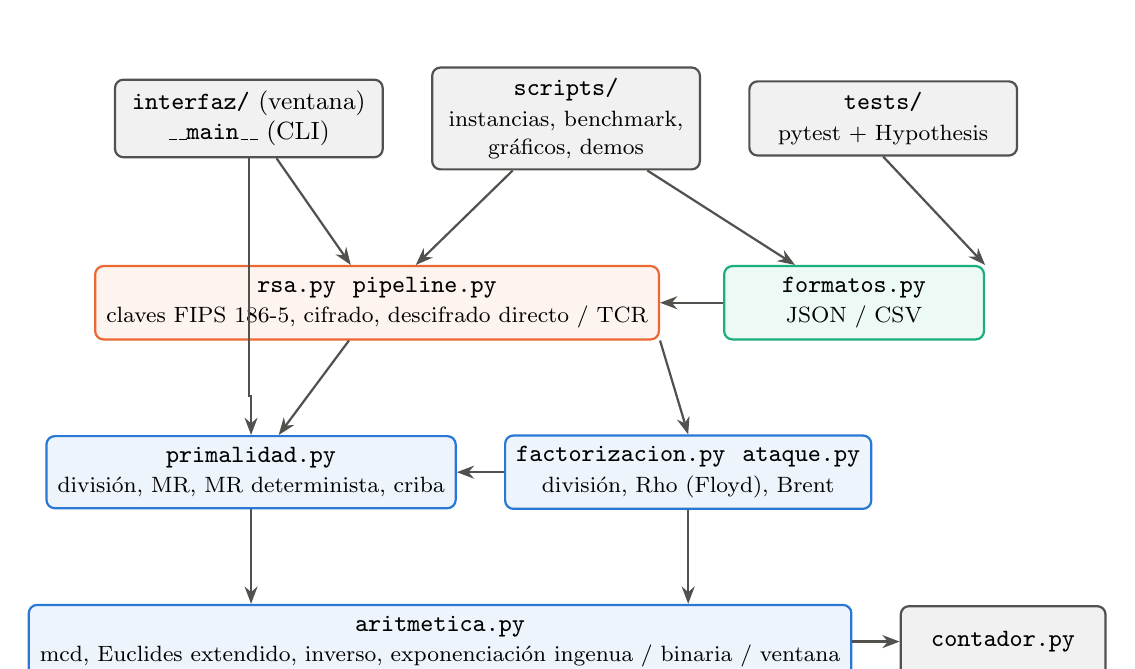
\begin{tikzpicture}[node distance=7mm and 6mm]
  \node[mod=gris, minimum width=3.4cm] (cli) {\texttt{interfaz/} (ventana)\\ \texttt{\_\_main\_\_} (CLI)};
  \node[mod=gris, minimum width=3.4cm, right=of cli] (scripts)
       {\texttt{scripts/}\\ \footnotesize instancias, benchmark,\\[-1pt]\footnotesize gráficos, demos};
  \node[mod=gris, minimum width=3.4cm, right=of scripts] (tests)
       {\texttt{tests/}\\ \footnotesize pytest + Hypothesis};
  \node[mod=naranja, minimum width=5.6cm, below=12mm of scripts, xshift=-2.4cm] (rsa)
       {\texttt{rsa.py} \ \texttt{pipeline.py}\\ \footnotesize claves FIPS 186-5, cifrado, descifrado directo / TCR};
  \node[mod=verde, minimum width=3.3cm, right=8mm of rsa] (fmt)
       {\texttt{formatos.py}\\ \footnotesize JSON / CSV};
  \node[mod, minimum width=4.4cm, below=12mm of rsa, xshift=-1.6cm] (prim)
       {\texttt{primalidad.py}\\ \footnotesize división, MR, MR determinista, criba};
  \node[mod, minimum width=4.4cm, right=6mm of prim] (fact)
       {\texttt{factorizacion.py} \ \texttt{ataque.py}\\ \footnotesize división, Rho (Floyd), Brent};
  \node[mod, minimum width=9.2cm, below=12mm of prim, xshift=2.4cm] (arit)
       {\texttt{aritmetica.py}\\ \footnotesize mcd, Euclides extendido, inverso, exponenciación ingenua / binaria / ventana};
  \node[mod=gris, minimum width=2.6cm, right=6mm of arit] (cont) {\texttt{contador.py}};

  \draw[flecha] (cli) -- (rsa);
  \draw[flecha] (cli.south) |- ($(prim.north)+(0,5mm)$) -- (prim.north);
  \draw[flecha] (scripts) -- (rsa);
  \draw[flecha] (scripts) -- (fmt);
  \draw[flecha] (tests.south) -- (fmt.north east);
  \draw[flecha] (rsa) -- (prim);
  \draw[flecha] (fmt) -- (rsa);
  \draw[flecha] (rsa.south east) -- (fact.north);
  \draw[flecha] (fact) -- (prim);
  \draw[flecha] (prim) -- (prim |- arit.north);
  \draw[flecha] (fact) -- (fact |- arit.north);
  \draw[flecha] (arit) -- (cont);
\end{tikzpicture}
\caption{Arquitectura en capas de \texttt{rsa\_edu}. Las flechas indican
«depende de». Gris: interfaz y soporte; naranja: aplicación integradora;
azul: algoritmos; verde: entrada/salida.}
\label{fig:arquitectura}
\end{figure}

\subsection{Módulos}

\begin{table}[H]
\centering\small
\caption{Módulos, responsables y funciones públicas (versión 0.2.0).}
\label{tab:modulos}
\begin{tabularx}{\textwidth}{@{}l l Y@{}}
\toprule
\textbf{Módulo} & \textbf{Resp.} & \textbf{Funciones principales}\\
\midrule
\texttt{aritmetica} & Francesco & \texttt{mcd}, \texttt{mcm}, \texttt{euclides\_extendido}, \texttt{inverso\_modular}, \texttt{exp\_modular\_ingenua}, \texttt{exp\_modular\_rapida}, \texttt{exp\_modular\_ventana}, \texttt{ventana\_optima}\\
\texttt{contador} & Francesco & \texttt{Contador} (multiplicaciones, divisiones, mcd, iteraciones)\\
\texttt{primalidad} & Orlando & \texttt{division\_tentativa}, \texttt{miller\_rabin}, \texttt{miller\_rabin\_determinista}, \texttt{es\_primo}, \texttt{es\_testigo}, \texttt{criba\_eratostenes}, \texttt{pasa\_criba}, \texttt{generar\_primo}\\
\texttt{factorizacion} & Camila & \texttt{factorizar\_tentativa}, \texttt{pollard\_rho}, \texttt{pollard\_rho\_brent}, \texttt{factorizar} (fachada)\\
\texttt{ataque} & Camila & \texttt{romper\_clave}: factoriza $n$ y recupera $d$\\
\texttt{rsa} & Emmi & \texttt{generar\_claves}, \texttt{generar\_claves\_aleatorias}, \texttt{elegir\_e}, \texttt{lambda\_carmichael}, \texttt{cifrar}, \texttt{descifrar}, \texttt{descifrar\_crt}, \texttt{cifrar\_texto}, \texttt{descifrar\_texto}\\
\texttt{pipeline} & Emmi & \texttt{ConfigPipeline}, \texttt{ejecutar\_pipeline}, \texttt{configuraciones\_estandar}\\
\texttt{formatos} & Emmi & \texttt{cargar\_instancias}, \texttt{guardar\_instancias}, \texttt{cargar\_claves}, \texttt{guardar\_claves}, \texttt{escribir\_resultados}, \texttt{leer\_resultados}\\
\texttt{\_\_main\_\_} & Emmi & CLI: \texttt{primo}, \texttt{factorizar}, \texttt{claves}, \texttt{cifrar}, \texttt{descifrar}, \texttt{atacar}, \texttt{comparar}, \texttt{pipeline}, \texttt{interfaz}\\
\texttt{interfaz} & Todos & Ventana con cinco pestañas: RSA y Optimización (Emmi), Exponenciación modular (Francesco), Primalidad (Orlando), Factorización y ataque (Camila); \texttt{comun} y \texttt{componentes} (Emmi)\\
\bottomrule
\end{tabularx}
\end{table}

\subsection{Formatos de archivos}

En JSON, los enteros grandes se guardan como \emph{cadenas decimales}; todo
archivo incluye un campo \texttt{version} y se \textbf{valida al cargarse}
(campos obligatorios, coherencia entre \texttt{n} y \texttt{bits}, consistencia
de la clave: $n = pq$ y $e\,d \equiv 1 \pmod{\lambda(n)}$).

\begin{lstlisting}[style=datos, caption={Instancias (\texttt{data/instancias/semiprimos.json}, extracto real).}]
{"version": 1,
 "meta": {"tipo": "semiprimo_balanceado",
          "generador": "scripts/generar_instancias.py --semilla 2026", "semilla": 2026},
 "instancias": [{"n": "47561", "bits": 16, "p": "199", "q": "239"}, ...]}
\end{lstlisting}

\begin{lstlisting}[style=datos, caption={Par de claves (\texttt{clave.json}, generado por la CLI).}]
{"version": 1, "tipo": "rsa-edu",
 "publica": {"n": "3233", "e": "17"},
 "privada": {"d": "2753", "p": "61", "q": "53"}}
\end{lstlisting}

\begin{lstlisting}[style=datos, caption={Resultados (\texttt{resultados/<configuración>/E1.csv} \dots{} \texttt{E6.csv}): columnas.}]
experimento,algoritmo,etapa,instancia,bits,repeticiones,
ms_mediana,ms_min,ms_max,cv,mult_mod,div_mod,mcd,iteraciones,
kib_pico,extra,ok,estable
\end{lstlisting}

\subsection{Dependencias}

\begin{table}[H]
\centering\small
\caption{Dependencias (\texttt{requirements.txt}). El núcleo no requiere ninguna.}
\begin{tabularx}{\textwidth}{@{}l l Y@{}}
\toprule
\textbf{Paquete} & \textbf{Versión mínima} & \textbf{Uso}\\
\midrule
Python & 3.10 & Lenguaje (probado con 3.10, 3.12 y 3.13 en Linux y Windows)\\
tkinter & incluido en Python & Interfaz gráfica\\
pytest, pytest-cov & 8.0, 5.0 & Pruebas y cobertura\\
hypothesis & 6.100 & Pruebas basadas en propiedades\\
sympy & 1.12 & Oráculo de referencia en pruebas y experimentos\\
pandas, matplotlib & 2.0, 3.7 & Tablas y figuras de resultados\\
gmpy2 (opcional) & 2.1 & Prototipo y \emph{backend} opcional del pipeline\\
\bottomrule
\end{tabularx}
\end{table}

\subsection{Decisiones técnicas}

\begin{table}[H]
\centering\small
\caption{Cambios introducidos al implementar.}
\label{tab:cambios}
\renewcommand{\arraystretch}{1.2}
\begin{tabularx}{\linewidth}{@{}R{3.4cm} R{4.2cm} Y@{}}
\toprule
\textbf{Diseño inicial} & \textbf{Implementado} & \textbf{Motivo}\\
\midrule
Pollard Rho sin límite & \texttt{max\_iter} y \texttt{max\_reintentos} & Con factores grandes podía no terminar; ahora lanza \texttt{RuntimeError} con un mensaje claro.\\
Rho aplicado a cualquier $n$ & Se detectan antes $n$ par y $n$ cuadrado perfecto & Para $n=r^2$ el mcd da $n$ con mucha frecuencia.\\
Recursión sobre los cofactores & Pila explícita & Evita el límite de recursión de Python.\\
Cofactores con MR aleatorio & \texttt{es\_primo}: MR determinista bajo $3{,}18\times10^{23}$ & Exacto y más rápido en ese rango.\\
$d$ siempre con $\varphi(n)$ & $\varphi(n)$ en claves manuales; $\lambda(n)$ en aleatorias & FIPS 186-5 (Tabla~\ref{tab:estandares}).\\
\texttt{generar\_primo} en \texttt{rsa.py} & Movido a \texttt{primalidad.py} con criba opcional & Pertenece a la capa de primalidad; permite comparar con y sin criba.\\
Una sola semilla para todo & Generador derivado para las bases de MR & Con y sin criba se obtiene el mismo primo: comparación justa.\\
Medición solo con tiempo & Parámetro opcional \texttt{cont} & Comparar por operaciones, independiente del hardware.\\
Experimentos E1--E4 & E1--E6 (se agregan criba y pipeline completo) & Responder directamente si se optimiza el RSA completo.\\
\bottomrule
\end{tabularx}
\end{table}

Otras decisiones: \texttt{\_\_init\_\_.py} no reexporta funciones, para que cada
integrante pueda subir su módulo sin romper las importaciones de los demás;
todas las funciones validan tipos y rangos (\texttt{bool} se rechaza
explícitamente, porque en Python es subclase de \texttt{int}).

% ================================================================== 8
\section{Estrategia de pruebas}
\label{sec:pruebas}

\subsection{Organización de la batería de pruebas}

La suite tiene \textbf{397 pruebas automatizadas} en 15 archivos, uno por
componente. Todas pasan, con \textbf{94\,\%} de cobertura de líneas. Se ejecutan
con \texttt{python -m pytest} y en GitHub Actions (Ubuntu y Windows, Python 3.10,
3.12 y 3.13) en cada \emph{push}.

\begin{table}[H]
\centering\small
\caption{Archivos de prueba, identificadores, casos y tipo de prueba.}
\label{tab:archivos-prueba}
\begin{tabularx}{\linewidth}{@{}l l r R{2.3cm} Y@{}}
\toprule
\textbf{Archivo} & \textbf{IDs} & \textbf{Casos} & \textbf{Tipo} & \textbf{Componente}\\
\midrule
\texttt{test\_aritmetica.py} & A1--A8 & 47 & Unitarias & mcd, Bézout, inverso, exponenciaciones, ventana, contador\\
\texttt{test\_primalidad.py} & P1--P11 & 94 & Unitarias & división, Miller--Rabin, MR determinista, criba, \texttt{generar\_primo}\\
\texttt{test\_factorizacion.py} & F1--F9 & 76 & Unitarias & división, Rho, Brent, \texttt{factorizar}, ataque\\
\texttt{test\_rsa.py} & R1--R12 & 52 & Unitarias & claves manuales y FIPS 186-5, cifrado, descifrado, TCR, texto\\
\texttt{test\_formatos.py} & R9 & 19 & Unitarias & instancias, claves y resultados (JSON, CSV)\\
\texttt{test\_propiedades.py} & -- & 7 & Propiedades & Bézout, inverso, ida y vuelta RSA, factorización, primo determinista\\
\texttt{test\_integracion.py} & I1--I6 & 21 & Integración & pipeline, CLI, entradas inválidas, scripts\\
\texttt{test\_demo\_optimizacion.py} & I7 & 5 & Integración & base y optimizado dan el mismo resultado\\
\texttt{test\_experimentos.py} & X1--X6 & 12 & Integración & formato, corrección y reproducibilidad del benchmark\\
\texttt{test\_interfaz\_comun.py} & G1 & 16 & Unitarias & lectura de entradas y comparación de alternativas en la interfaz\\
\texttt{test\_interfaz\_exponenciacion.py} & G2 & 9 & Unitarias & pestaña de exponenciación y paso a paso de la binaria\\
\texttt{test\_interfaz\_primalidad.py} & G3 & 10 & Unitarias & pestaña de primalidad y generación de primos\\
\texttt{test\_interfaz\_factorizacion.py} & G4 & 10 & Unitarias & pestaña de factorización y ataque\\
\texttt{test\_interfaz\_rsa.py} & G5 & 9 & Unitarias & pestañas RSA y Optimización\\
\texttt{test\_interfaz\_ventana.py} & G6 & 10 & Integración & la ventana completa: cada botón muestra el resultado correcto\\
\midrule
\textbf{Total} & & \textbf{397} & & \\
\bottomrule
\end{tabularx}
\end{table}

\subsection{Casos normales, límite, adversos, aleatorios y de referencia}

\begin{table}[H]
\centering
\caption{Cobertura de cada componente por tipo de caso (identificadores de prueba).}
\label{tab:bateria}
\scriptsize
\renewcommand{\arraystretch}{1.25}
\begin{tabularx}{\linewidth}{@{}R{1.9cm} Y Y Y Y Y@{}}
\toprule
\textbf{Componente} & \textbf{Normal} & \textbf{Límite} & \textbf{Adverso} & \textbf{Aleatorio con semilla} & \textbf{Referencia}\\
\midrule
Aritmética & A1--A3: $17^{-1}\bmod3120=2753$ & A4: exponente 0, módulo 1; A5: $k=1..8$ & A6: negativos, módulo $\le0$, $k$ inválido & Bézout e inverso (Hypothesis) & \texttt{pow} de Python; traza manual (A2)\\
Primalidad & P5: primos conocidos & P2: $n\in\{0,1,2,3\}$; P11: límite $3{,}18\times10^{23}$ & P3: Carmichael; P4: pseudoprimos fuertes ($2047$, \dots) & P10: \texttt{generar\_primo} con semillas; Hypothesis & \textbf{exhaustiva}: $n\in[0,20\,000]$ frente a \texttt{sympy.isprime} (P1); P8: cota de $1/4$\\
Factorización & F1: $3233$, $600\,851\,475\,143$ & F6: cuadrados de primos, potencias, $2^{61}-1$ & F7: $n\le0$, método desconocido, \texttt{max\_iter} agotado & F3: enteros de 60 bits; F5: semiprimos hasta 80 bits & \textbf{exhaustiva}: $[1,3000]$ frente a \texttt{sympy.factorint} (F2); cruzada (F4)\\
RSA & R1: ejemplo manual; R3: ida y vuelta 16--2048 bits & R7: $m\in\{0,1,n-1\}$; R8: texto vacío & R10: $p=q$, $e$ no invertible, $m\ge n$, \texttt{True} & R4: claves FIPS reproducibles; Hypothesis & \textbf{exhaustiva}: los 3233 mensajes de la clave manual (R2)\\
Formatos & R9: guardar y leer & R9: solo clave pública & R9: JSON mal formado, clave alterada & -- & valores conocidos\\
Integración & I1: 6 configuraciones; I7 & I1: mensajes en el borde del rango & I4: entradas inválidas en la CLI & I1: misma clave con la misma semilla & \texttt{pow} y mensaje original\\
Interfaz & G2--G5: ejemplo del informe en cada pestaña & G2: exponente 0, módulo 1; G3: $n \ge 2^{48}$ omite la división & G1: textos no numéricos; G5: $m \ge n$, criptograma vacío & G2--G4: números aleatorios con semilla & \texttt{pow} de Python; G6: ventana completa\\
Experimentos & X1: formato de CSV & X5: carpeta sin datos & X5: experimento desconocido, configuración incompleta & X3: dos corridas, mismos conteos & X2: \texttt{sympy} y \texttt{pow} en cada fila\\
\bottomrule
\end{tabularx}
\end{table}

\lstinputlisting[style=datos, caption={Salida de \texttt{python -m pytest --cov=rsa\_edu}.}]{salidas/pytest.txt}

\subsection{Cómo se verifica que las salidas son correctas}

Se hacen dos comparaciones con propósitos distintos:

\begin{table}[H]
\centering\small
\caption{Qué se compara con qué.}
\label{tab:comparaciones}
\renewcommand{\arraystretch}{1.25}
\begin{tabularx}{\linewidth}{@{}R{2.5cm} Y Y@{}}
\toprule
& \textbf{1. Corrección} & \textbf{2. Eficiencia (optimización)}\\
\midrule
Pregunta & ¿Nuestros algoritmos dan el resultado correcto? & ¿La segunda alternativa es más rápida que la primera?\\
Se compara & Nuestro resultado contra una \textbf{implementación de referencia externa} y contra la definición & Nuestra primera alternativa contra nuestra segunda alternativa, sobre las mismas instancias\\
Referencias & \texttt{pow(b, e, m)} de Python (en C), \texttt{sympy.isprime}, \texttt{sympy.factorint}, \texttt{gmpy2.powmod}; valores conocidos (ejemplo manual, Carmichael, pseudoprimos fuertes) & Contador de operaciones y tiempo medido\\
Dónde & \texttt{tests/}, columna \texttt{ok} de cada experimento, demos & \texttt{benchmark.py}, \texttt{comparar}, \texttt{demo\_optimizacion.py}\\
\bottomrule
\end{tabularx}
\end{table}

Los algoritmos de la biblioteca no usan estas referencias: \texttt{sympy} y
\texttt{pow} con tres argumentos aparecen solo en pruebas, experimentos y demos.
La única biblioteca externa que el sistema puede usar en su ejecución es
\texttt{gmpy2}, de forma opcional en \texttt{pipeline.py}; la prueba I1 verifica
que esa configuración produce la misma clave y los mismos cifrados que la
nuestra. La eficiencia no se juzga contra una biblioteca escrita en C, porque la
diferencia reflejaría el lenguaje y no el algoritmo; por eso las dos alternativas
comparadas son implementaciones propias en las mismas condiciones.

A estas comparaciones se suman otros tres mecanismos:
\begin{itemize}
  \item \textbf{Invariantes de salida}, que no necesitan oráculo (Tabla~\ref{tab:invariantes}).
  \item \textbf{Pruebas basadas en propiedades (Hypothesis)}: se declara una
        propiedad («para todo $m$: descifrar(cifrar($m$)) $= m$») y la herramienta
        genera cientos de entradas y reduce cualquier fallo al contraejemplo mínimo.
  \item \textbf{Verificación estadística} de los algoritmos probabilísticos: la
        tasa de error de Miller--Rabin con una ronda queda bajo la cota de $1/4$ (P8).
\end{itemize}

\begin{table}[H]
\centering\small
\caption{Invariantes que se comprueban automáticamente.}
\label{tab:invariantes}
\begin{tabularx}{\textwidth}{@{}l Y@{}}
\toprule
\textbf{Módulo} & \textbf{Invariante}\\
\midrule
Euclides extendido & $a x + b y = g$, $g \mid a$ y $g \mid b$\\
Inverso modular & $a \cdot a^{-1} \equiv 1 \pmod m$ y $0 < a^{-1} < m$\\
Exponenciación & coincide con \texttt{pow}; la binaria hace a lo sumo $2\lfloor\log_2 e\rfloor + 1$ multiplicaciones; la ventana, menos\\
Factorización & $\prod F = n$, todo $f \in F$ es primo y $F$ está ordenada\\
Pollard Rho y Brent & si devuelve $d$, entonces $1 < d < n$ y $d \mid n$\\
Claves & $n = pq$, $p \ne q$ primos, $e d \equiv 1 \pmod{\lambda(n)}$; las aleatorias cumplen FIPS 186-5\\
Cifrado & $\textsc{Descifrar}(\textsc{Cifrar}(m)) = \textsc{DescifrarTCR}(\textsc{Cifrar}(m)) = m$\\
\bottomrule
\end{tabularx}
\end{table}

\subsection{Validación con la instancia resuelta a mano}

La instancia de la Sección~\ref{sec:instancia} se reproduce exactamente. El
script \texttt{scripts/traza\_instancia.py} muestra la tabla de Euclides
extendido, la traza de la exponenciación y el descifrado por TCR, y compara cada
valor con \texttt{pow}:

\lstinputlisting[style=datos, caption={Salida de \texttt{python scripts/traza\_instancia.py}.}]{salidas/traza.txt}

Durante la sesión se puede proponer cualquier instancia; el script verifica por
sí mismo cada resultado, y rechaza las inválidas:

\lstinputlisting[style=datos, caption={Salida de \texttt{python scripts/traza\_instancia.py --p 61 --q 51}.}]{salidas/inval1.txt}

\subsection{Equivalencia entre alternativas}

\lstinputlisting[style=datos, caption={Las alternativas de cada etapa sobre la misma instancia (\texttt{python -m rsa\_edu comparar}).}]{salidas/comparar.txt}

\begin{table}[H]
\centering\small
\caption{Resultados de ambas alternativas sobre las mismas instancias.}
\begin{tabularx}{\linewidth}{@{}l Y Y c@{}}
\toprule
\textbf{Instancia} & \textbf{Primera alternativa} & \textbf{Segunda alternativa} & \textbf{¿Coinciden?}\\
\midrule
$65^{17}\bmod3233$ & binaria: 2790 & ventana: 2790 & sí\\
$561$, $2047$ & división: compuestos & MR y MR determinista: compuestos & sí\\
$n=3233$ & división: $[53, 61]$ & Rho y Brent: $[53, 61]$ & sí\\
$2^{32}+1$ & división: $[641, 6700417]$ & Rho y Brent: $[641, 6700417]$ & sí\\
Descifrar $2790$ & directo: 65 & TCR: 65 & sí\\
Primo de 512 bits, semilla 7 & sin criba: $12161158388\ldots$ & con criba: $12161158388\ldots$ & sí, el mismo\\
\bottomrule
\end{tabularx}
\end{table}

\begin{table}[H]
\centering\small
\caption{Diferencias observadas entre alternativas y su explicación.}
\label{tab:diferencias}
\renewcommand{\arraystretch}{1.2}
\begin{tabularx}{\linewidth}{@{}R{4.3cm} Y R{2.6cm}@{}}
\toprule
\textbf{Diferencia} & \textbf{Explicación} & \textbf{Tipo}\\
\midrule
Binaria usa 6 multiplicaciones y ventana 5 ($e=17$) & El valor es el mismo; cambia el trabajo, que es lo que se mide. & Propiedad esperada\\
Pollard Rho devuelve 53 o 61 según la semilla & Es aleatorizado; \texttt{factorizar} ordena la lista y el resultado final es idéntico. & Decisión de implementación\\
MR con la sola base 2 declara primo a $2047=23\cdot89$ & $2047$ es pseudoprimo fuerte en base 2; con bases aleatorias o la base 3 se detecta. & Propiedad esperada\\
$d=2753$ con $\varphi(n)$; $d=413$ con $\lambda(n)$ & $\lambda(n)$ divide a $\varphi(n)$; ambos descifran $2790\rightarrow65$. & Decisión (FIPS 186-5)\\
Con $n=3233$ el TCR no es más rápido & Con claves diminutas pesa el costo fijo de reducir y recombinar; la ventaja aparece desde 512 bits. & Propiedad esperada\\
Con $\le24$ bits la división de prueba gana a MR & $\sqrt n$ es pequeño y MR tiene un costo fijo de 20 rondas. & Propiedad esperada\\
\bottomrule
\end{tabularx}
\end{table}

Ninguna diferencia corresponde a un error pendiente. La equivalencia se comprueba
automáticamente en cada \emph{push} (pruebas P1, F2, F4, A4, R2, R6, I1 e I7).

\subsection{Semillas y reproducibilidad}

Todo lo aleatorio del proyecto usa una semilla fija (2026 por defecto): las
instancias (\texttt{scripts/\allowbreak generar\_instancias.py}, que registra la semilla en
el campo \texttt{meta} de cada archivo JSON), las configuraciones de los
experimentos (\texttt{config/*.json}), las pruebas (\texttt{tests/conftest.py}) y
las funciones de la biblioteca, que reciben el generador como parámetro
(\texttt{rng}). Con la misma semilla se obtienen las mismas instancias, las
mismas claves y los mismos conteos en cualquier computadora: regenerar las
instancias produce archivos idénticos byte a byte, y las pruebas R4, X3 y la
propiedad \texttt{test\_generar\_\allowbreak primo\_\allowbreak determinista} lo verifican.


% ================================================================== 9
\section{Metodología experimental}
\label{sec:metodologia}

\subsection{Preguntas de evaluación e hipótesis}

\begin{table}[H]
\centering\small
\caption{Preguntas de evaluación, hipótesis y experimento que las responde.}
\label{tab:preguntas}
\begin{tabularx}{\linewidth}{@{}l Y Y c@{}}
\toprule
\textbf{N.º} & \textbf{Pregunta} & \textbf{Hipótesis (según la teoría)} & \textbf{Exp.}\\
\midrule
Q1 & ¿Desde qué tamaño conviene Miller--Rabin frente a la división de prueba? & La división crece como $2^{b/2}$ y MR de forma polinomial: MR gana desde unas decenas de bits & E1\\
Q2 & ¿Cuánto más rápido factoriza Pollard Rho, y cuánto aporta Brent? & Rho crece como $2^{b/4}$ frente a $2^{b/2}$; Brent mantiene el orden con menor constante & E2\\
Q3 & ¿Cuántas multiplicaciones ahorra la ventana deslizante? & De $1{,}5$ a $\approx 1 + 1/(k+1)$ multiplicaciones por bit del exponente & E3\\
Q4 & ¿Cuánto acelera el TCR el descifrado? & Hasta 4 veces con multiplicación escolar; menos con claves pequeñas & E4\\
Q5 & ¿Cuántas pruebas de Miller--Rabin evita la criba? & $\approx 85\,\%$, por el teorema de Mertens, con el mismo primo resultante & E5\\
Q6 & ¿Cuánto se acelera el pipeline RSA completo? & Varias veces, concentrado en generar claves y descifrar; el cifrado no cambia & E6\\
\bottomrule
\end{tabularx}
\end{table}

\subsection{Instancias y tamaños}

\begin{table}[H]
\centering
\caption{Experimentos del diseño definitivo (\texttt{config/experimentos.json}).}
\label{tab:diseno}
\scriptsize
\renewcommand{\arraystretch}{1.25}
\begin{tabularx}{\linewidth}{@{}l R{2.3cm} R{3.2cm} R{3.0cm} Y@{}}
\toprule
\textbf{Exp.} & \textbf{Alternativas} & \textbf{Instancias} & \textbf{Tamaños} & \textbf{Verificación}\\
\midrule
E1 & división, MR (20 rondas), MR determinista & \texttt{primos.json} (peor caso) y \texttt{adversos.json} (Carmichael y pseudoprimos fuertes) & 8--512 bits; división hasta 48 & \texttt{sympy.isprime}\\
E2 & división, Rho, Brent & \texttt{semiprimos.json}: $p$ y $q$ de $b/2$ bits (peor caso de la división) & 16--64 bits; división hasta 48 & \texttt{sympy.factorint}\\
E3 & binaria, ventana & módulo, base y exponente aleatorios de $b$ bits (caso promedio), 5 por tamaño & 256, 512, 1024, 2048, 4096 & \texttt{pow}\\
E4 & directo, TCR & 3 claves FIPS 186-5 por tamaño, 10 mensajes por clave & 512, 1024, 2048, 4096 & mensaje original\\
E5 & sin criba, con criba & 5 semillas por tamaño (los mismos candidatos en ambas) & 256, 512, 1024, 2048 & \texttt{sympy.isprime}, mismo primo\\
E6 & pipeline base, optimizado & 3 semillas por tamaño, 10 mensajes & 512, 1024, 2048, 4096 & misma clave, \texttt{pow}, mensajes\\
\bottomrule
\end{tabularx}
\end{table}

\subsection{Variables y métricas}

\begin{itemize}
  \item \textbf{Variables independientes:} la alternativa (primera o segunda) y el tamaño de la entrada en bits.
  \item \textbf{Variables controladas:} las mismas instancias y semillas para todas las alternativas de
        un experimento (comparación pareada); el mismo equipo, intérprete y proceso; recolector de
        basura desactivado durante cada medición; parámetros por defecto fijos ($k$ óptimo, 20
        rondas, lotes de 128).
  \item \textbf{Métricas (variables dependientes):} tiempo en milisegundos (mediana, mínimo, máximo y
        coeficiente de variación de las repeticiones); multiplicaciones y divisiones modulares,
        llamadas a mcd e iteraciones (independientes del hardware); memoria pico con
        \texttt{tracemalloc}; llamadas a Miller--Rabin (E5); corrección (\texttt{ok}) y estabilidad
        entre repeticiones (\texttt{estable}).
\end{itemize}

\subsection{Entorno}

Las mediciones preliminares se ejecutaron con CPython~3.13.18 en Linux x86\_64,
en un solo proceso, con la versión 0.2.0 de la biblioteca. Cada corrida guarda
su entorno en \texttt{metadatos.json} (fecha, versión de Python, sistema,
procesador, commit, semilla y hash de la configuración), de modo que cada
resultado se puede rastrear hasta el código y la configuración que lo produjo.

\subsection{Procedimiento reproducible}

Para cada alternativa e instancia, \texttt{benchmark.medir} ejecuta:
\begin{enumerate}
  \item una ejecución de conteo, no cronometrada, con \texttt{Contador} y \texttt{tracemalloc};
        su resultado se verifica contra la referencia de la Tabla~\ref{tab:diseno};
  \item una ejecución de calentamiento, descartada;
  \item $R$ ejecuciones cronometradas con \texttt{time.perf\_counter}, sin contador y con el
        recolector de basura desactivado; cada una debe dar el mismo resultado que la de conteo;
  \item una fila con la mediana y el resto de las métricas.
\end{enumerate}
Las mejoras se calculan como la mediana, por tamaño, de los cocientes \emph{sobre
la misma instancia}, no como cociente de medianas. Los resultados se guardan en
un CSV por experimento y se procesan con \texttt{graficar.py} (tablas y figuras)
y \texttt{ajuste\_complejidad.py} (comparación con la teoría). Los comandos para
reproducir todo están en el Anexo~\ref{anx:uso}.

\begin{table}[H]
\centering\small
\caption{Tres configuraciones del mismo procedimiento.}
\begin{tabularx}{\linewidth}{@{}l c Y r@{}}
\toprule
\textbf{Configuración} & \textbf{Repeticiones} & \textbf{Tamaños} & \textbf{Duración}\\
\midrule
\texttt{piloto.json} & 3 & pequeños (E3 hasta 512, E4--E6 512 bits) & $\approx 7$\,s por corrida\\
\texttt{preliminar.json} & 3 & medianos (hasta 2048 bits; E5 hasta 1024) & $\approx 3{,}5$\,min\\
\texttt{experimentos.json} (definitivo) & 5 & completos (hasta 4096 bits) & más de 30\,min\\
\bottomrule
\end{tabularx}
\end{table}

\subsection{Experimento piloto}
\label{sec:piloto}

El piloto comprueba que el procedimiento produce datos \textbf{correctos,
coherentes y reproducibles} antes de las corridas grandes.
\texttt{scripts/verificar\_reproducibilidad.py} ejecuta la configuración piloto
dos veces y compara:

\begin{table}[H]
\centering\small
\caption{Resultado del piloto (\texttt{resultados/piloto/reproducibilidad.md}).}
\begin{tabularx}{\linewidth}{@{}Y r c@{}}
\toprule
\textbf{Comprobación} & \textbf{Resultado} & \\
\midrule
\multicolumn{3}{@{}l}{\textit{Correctos}}\\
Filas medidas por corrida & 184 & \\
Filas con resultado incorrecto o inestable & 0 & \checkmark\\
\multicolumn{3}{@{}l}{\textit{Reproducibles}}\\
Mismas filas en ambas corridas & sí & \checkmark\\
Filas con conteos de operaciones distintos & 0 & \checkmark\\
Tiempos con diferencia $\le 25\,\%$ entre corridas & 118/126 (94\,\%) & \checkmark\\
Diferencia relativa mediana entre corridas & 4,4\,\% & \\
Coeficiente de variación mediano dentro de una corrida & 5,6\,\% & \\
\multicolumn{3}{@{}l}{\textit{Coherentes con la teoría}}\\
E1: la división hace a lo más $\sqrt n/6+1$ iteraciones & 26/26 & \checkmark\\
E3: la binaria hace a lo más $2b$ multiplicaciones & 4/4 & \checkmark\\
E3: la ventana hace menos multiplicaciones que la binaria & 4/4 & \checkmark\\
E4: el TCR descifra en menos tiempo que el directo & 1/1 & \checkmark\\
E5: la criba reduce las llamadas a Miller--Rabin & 2/2 & \checkmark\\
E6: el cifrado hace las mismas multiplicaciones en base y optimizado & 1/1 & \checkmark\\
E6: el descifrado optimizado es más rápido que el base & 1/1 & \checkmark\\
\bottomrule
\end{tabularx}
\end{table}

Los conteos son exactamente reproducibles porque todo lo aleatorio depende de
semillas; los tiempos varían un poco entre corridas, como es normal. Las filas
por debajo de 50\,µs no se comparan, porque ahí domina el ruido del reloj.

% ================================================================== 10
\section{Resultados}
\label{sec:resultados}

\subsection{Primalidad y factorización (E1, E2)}

\subsection{Exponenciación y descifrado (E3, E4)}

\subsection{Generación de primos con y sin criba (E5)}

\subsection{Pipeline RSA completo (E6)}

\subsection{Costo de implementación: prototipo con \texttt{gmpy2}}

% ================================================================== 11
\section{Discusión crítica}
\label{sec:discusion}

\subsection{Contraste con el análisis teórico}

\subsection{Ventajas, limitaciones y situaciones en que conviene cada alternativa}

\subsection{Amenazas a la validez}

% ================================================================== 12
\section{Conclusiones y recomendaciones}
\label{sec:conclusiones}

\subsection{Respuesta a los objetivos}

\subsection{Síntesis de hallazgos}

\subsection{Lecciones aprendidas}

\subsection{Trabajo futuro}

% ================================================================== 13
\section{Referencias}
\label{sec:referencias}

\begingroup
\renewcommand{\section}[2]{}
\begin{thebibliography}{99}\small
\bibitem{clrs} T.~H. Cormen, C.~E. Leiserson, R.~L. Rivest y C.~Stein,
  \emph{Introduction to Algorithms}, 4.\textsuperscript{a} ed. MIT Press, 2022
  (cap.~31: algoritmos de teoría de números).
\bibitem{hac} A.~J. Menezes, P.~C. van Oorschot y S.~A. Vanstone,
  \emph{Handbook of Applied Cryptography}. CRC Press, 1996.
\bibitem{knuth} D.~E. Knuth, \emph{The Art of Computer Programming, Vol.~2:
  Seminumerical Algorithms}, 3.\textsuperscript{a} ed. Addison-Wesley, 1997.
\bibitem{rsa1978} R.~L. Rivest, A.~Shamir y L.~Adleman, «A method for obtaining
  digital signatures and public-key cryptosystems», \emph{Communications of the
  ACM}, vol.~21, n.º~2, pp.~120--126, 1978.
\bibitem{miller1976} G.~L. Miller, «Riemann's hypothesis and tests for
  primality», \emph{Journal of Computer and System Sciences}, vol.~13, n.º~3,
  pp.~300--317, 1976.
\bibitem{rabin1980} M.~O. Rabin, «Probabilistic algorithm for testing
  primality», \emph{Journal of Number Theory}, vol.~12, n.º~1, pp.~128--138, 1980.
\bibitem{pollard1975} J.~M. Pollard, «A Monte Carlo method for factorization»,
  \emph{BIT Numerical Mathematics}, vol.~15, n.º~3, pp.~331--334, 1975.
\bibitem{brent1980} R.~P. Brent, «An improved Monte Carlo factorization
  algorithm», \emph{BIT Numerical Mathematics}, vol.~20, n.º~2, pp.~176--184, 1980.
\bibitem{pomerance1980} C.~Pomerance, J.~L. Selfridge y S.~S. Wagstaff, «The
  pseudoprimes to $25\cdot10^9$», \emph{Mathematics of Computation}, vol.~35,
  n.º~151, pp.~1003--1026, 1980.
\bibitem{sorenson2017} J.~Sorenson y J.~Webster, «Strong pseudoprimes to twelve
  prime bases», \emph{Mathematics of Computation}, vol.~86, n.º~304,
  pp.~985--1003, 2017.
\bibitem{qc1982} J.-J. Quisquater y C.~Couvreur, «Fast decipherment algorithm
  for RSA public-key cryptosystem», \emph{Electronics Letters}, vol.~18, n.º~21,
  pp.~905--907, 1982.
\bibitem{rfc8017} K.~Moriarty, B.~Kaliski, J.~Jonsson y A.~Rusch,
  «PKCS \#1: RSA Cryptography Specifications Version 2.2», RFC~8017, IETF, 2016.
\bibitem{fips186} NIST, \emph{Digital Signature Standard (DSS)}, FIPS~186-5, 2023.
\bibitem{hypothesis} D.~R. MacIver, Z.~Hatfield-Dodds et~al., «Hypothesis: A new
  approach to property-based testing», \emph{Journal of Open Source Software},
  vol.~4, n.º~43, p.~1891, 2019.
\bibitem{pydocs} Python Software Foundation, documentación de los módulos
  \texttt{secrets}, \texttt{random}, \texttt{time} y \texttt{tracemalloc}.
  \url{https://docs.python.org/3/library/}
\bibitem{gmpy2} Documentación de gmpy2. \url{https://gmpy2.readthedocs.io}
\bibitem{pytest} Documentación de pytest. \url{https://docs.pytest.org}
\bibitem{nist80057} E.~Barker, \emph{Recommendation for Key Management: Part 1 -- General},
  NIST Special Publication 800-57 Part~1 Rev.~5, 2020.
\bibitem{aks2004} M.~Agrawal, N.~Kayal y N.~Saxena, «PRIMES is in P», \emph{Annals of Mathematics},
  vol.~160, n.º~2, pp.~781--793, 2004.
\bibitem{dlp1993} I.~Damgård, P.~Landrock y C.~Pomerance, «Average case error estimates for the
  strong probable prime test», \emph{Mathematics of Computation}, vol.~61, n.º~203, pp.~177--194, 1993.
\bibitem{bw1980} R.~Baillie y S.~S. Wagstaff, «Lucas pseudoprimes», \emph{Mathematics of
  Computation}, vol.~35, n.º~152, pp.~1391--1417, 1980.
\bibitem{lenstra1987} H.~W. Lenstra, «Factoring integers with elliptic curves», \emph{Annals of
  Mathematics}, vol.~126, n.º~3, pp.~649--673, 1987.
\bibitem{boudot2020} F.~Boudot, P.~Gaudry, A.~Guillevic, N.~Heninger, E.~Thomé y P.~Zimmermann,
  «Comparing the difficulty of factorization and discrete logarithm: a 240-digit experiment», en
  \emph{Advances in Cryptology -- CRYPTO 2020}, LNCS~12171, pp.~62--91, Springer, 2020.
\bibitem{progit} S.~Chacon y B.~Straub, \emph{Pro Git}, 2.\textsuperscript{a} ed. Apress, 2014.
  \url{https://git-scm.com/book}
\bibitem{pypa} Python Packaging Authority, \emph{Python Packaging User Guide}.
  \url{https://packaging.python.org}
\end{thebibliography}
\endgroup

\newpage

% ================================================================== 14
\section{Anexos}
\label{sec:anexos}

% ------------------------------------------------------------------ A
\subsection{Anexo A. Manual de instalación}
\label{anx:instalacion}

\paragraph{Requisitos.} Python 3.10 o superior y Git. Probado con Python 3.10,
3.12 y 3.13 en Linux y Windows.

\paragraph{Windows con Visual Studio Code.}
\begin{enumerate}
  \item Comprobar Python con \texttt{py --version}. Si no responde, instalar Python
        desde \url{https://www.python.org/downloads/} marcando
        \emph{Add python.exe to PATH}, y reabrir VS Code.
  \item Abrir la carpeta \texttt{ProyectoAlgoritmos} (\emph{Archivo $\rightarrow$
        Abrir carpeta}) y una terminal (\emph{Terminal $\rightarrow$ Nueva terminal}).
  \item Instalar las dependencias y la biblioteca:
\begin{lstlisting}[style=datos]
py -m pip install -r requirements.txt
py -m pip install -e .
py -m rsa_edu --version          # debe responder: rsa_edu 0.2.0
\end{lstlisting}
  \item Si \texttt{gmpy2} no se instala, instalar el resto: es opcional.
  \item La interfaz gráfica usa Tkinter, que viene con el instalador de
        python.org (opción \emph{tcl/tk and IDLE}, marcada por defecto).
\end{enumerate}

\paragraph{Linux o macOS.}\mbox{}
\begin{lstlisting}[style=datos]
git clone https://github.com/kita-02/ProyectoAlgoritmos.git
cd ProyectoAlgoritmos
python3 -m venv .venv && source .venv/bin/activate
pip install -r requirements.txt && pip install -e .
python -m pytest                 # debe terminar con: 397 passed
\end{lstlisting}

% ------------------------------------------------------------------ B
\subsection{Anexo B. Manual de uso}
\label{anx:uso}

En Windows se escribe \texttt{py} en lugar de \texttt{python}.

\paragraph{Interfaz gráfica.} Se abre con \texttt{python -m rsa\_edu interfaz}
(o \texttt{python -m rsa\_edu.interfaz}). Tiene cinco pestañas: \emph{RSA}
(generar claves, cifrar y descifrar de forma directa o con el TCR),
\emph{Exponenciación modular}, \emph{Primalidad}, \emph{Factorización y ataque}
y \emph{Optimización}, que ejecuta el pipeline base y el optimizado con la misma
semilla. Cada pestaña muestra los resultados en tablas con el tiempo y las
operaciones de cada alternativa, y una línea verde ($\checkmark$) o roja ($\times$) que indica si
todas dieron el mismo resultado. La semilla de la parte superior hace que los
datos aleatorios sean reproducibles.

\begin{figure}[H]
\centering
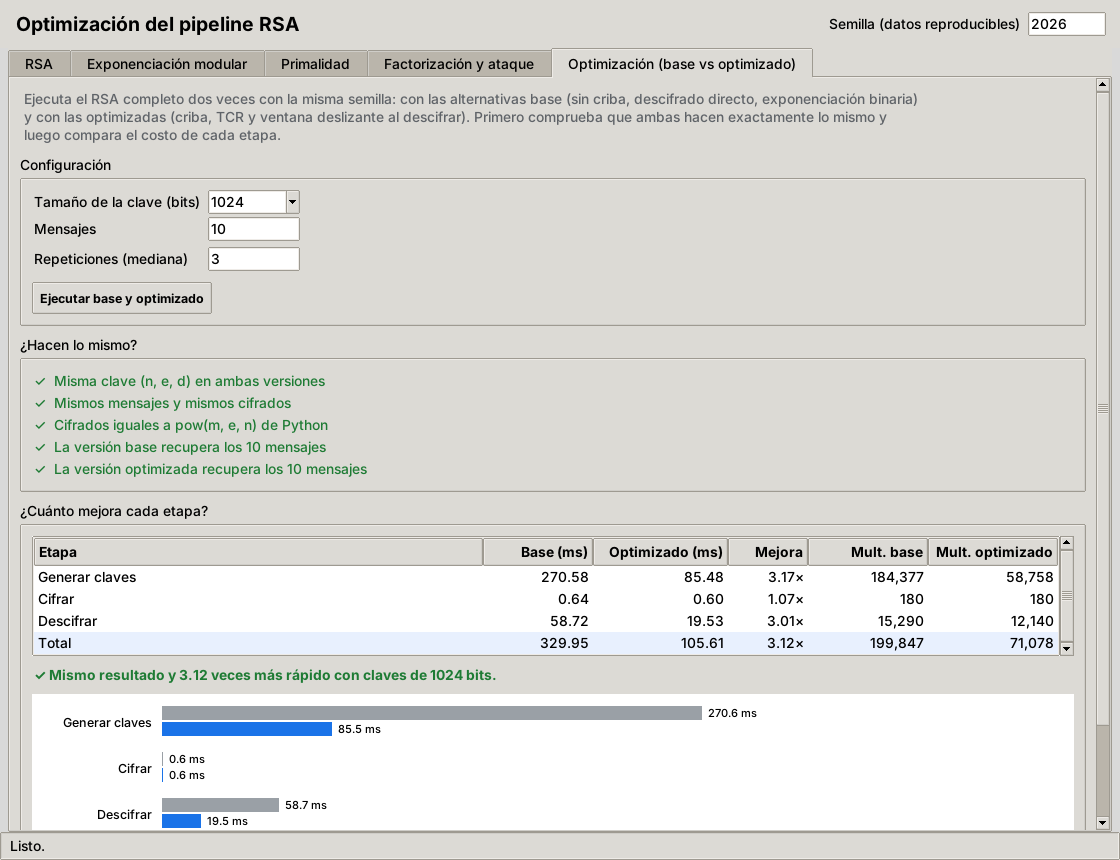
\includegraphics[width=0.9\linewidth]{figuras/interfaz_optimizacion.png}
\caption{Pestaña \emph{Optimización} de la interfaz gráfica (clave de 1024 bits).}
\label{fig:interfaz}
\end{figure}

\paragraph{Línea de comandos.}

\begin{table}[H]
\centering\small
\caption{Subcomandos de la línea de comandos (\texttt{python -m rsa\_edu}).}
\label{tab:cli}
\begin{tabularx}{\linewidth}{@{}>{\ttfamily\footnotesize}R{7.8cm} Y@{}}
\toprule
\textrm{\textbf{Comando}} & \textbf{Qué hace}\\
\midrule
primo 561 [--metodo tentativa | mr | determinista] & Decide si $n$ es primo con el método elegido\\
primo --generar 512 --semilla 7 [--sin-criba] & Genera un primo de 512 bits (con o sin criba)\\
factorizar 3233 --metodo tentativa | rho | brent & Factoriza $n$\\
claves -p 61 -q 53 -e 17 --salida clave.json & Crea la clave del ejemplo manual\\
claves --bits 1024 --salida c.json & Genera una clave según FIPS 186-5\\
cifrar 65 --claves clave.json [--ventana] & Cifra un entero (o \texttt{--texto "..."})\\
descifrar 2790 --claves clave.json [--crt] & Descifra, directo o por TCR\\
atacar -n 3233 -e 17 & Factoriza $n$ y recupera la clave privada\\
comparar primalidad | factorizacion | exponenciacion | descifrado X & Ejecuta todas las alternativas sobre la misma instancia\\
pipeline --bits 1024 [--crt] [--ventana] [--sin-criba] [--gmpy2] & Claves $\rightarrow$ cifrado $\rightarrow$ descifrado con métricas\\
interfaz & Abre la interfaz gráfica\\
\bottomrule
\end{tabularx}
\end{table}

\begin{table}[H]
\centering\small
\caption{Scripts de demostración y de experimentos.}
\begin{tabularx}{\linewidth}{@{}>{\ttfamily\footnotesize}R{7.8cm} Y@{}}
\toprule
\textrm{\textbf{Comando}} & \textbf{Qué hace}\\
\midrule
python scripts/traza\_instancia.py [--p P --q Q --e E --m M] & Traza paso a paso del ejemplo manual, con TCR\\
python scripts/demo\_primalidad.py 61 561 2047 & Compara división, MR y MR determinista\\
python scripts/demo\_factorizacion.py 3233 8051 & Compara división, Rho y Brent\\
python scripts/demo\_optimizacion.py [--bits 2048] & Pipeline base frente a optimizado, mismo resultado\\
python scripts/prototipo\_gmpy2.py & Binaria, ventana, \texttt{pow} y \texttt{gmpy2}\\
python scripts/generar\_instancias.py & Regenera \texttt{data/instancias/} con semilla 2026\\
python scripts/verificar\_reproducibilidad.py & Experimento piloto (dos corridas)\\
python scripts/benchmark.py --config config/preliminar.json & Experimentos preliminares E1--E6\\
python scripts/graficar.py resultados/preliminar & Figuras y tablas\\
python scripts/ajuste\_complejidad.py resultados/preliminar & Teoría frente a mediciones\\
python -m pytest [--cov=rsa\_edu] & Pruebas automatizadas (y cobertura)\\
\bottomrule
\end{tabularx}
\end{table}

\lstinputlisting[style=datos, caption={Flujo completo con la CLI: clave, cifrado, descifrado y ataque.}]{salidas/cli_validos.txt}

% ------------------------------------------------------------------ C
\subsection{Anexo C. Bitácora resumida del grupo}
\label{anx:bitacora}

La bitácora completa está en \texttt{docs/BITACORA\_GRUPAL.md}. Las fechas
corresponden a los commits del repositorio y a las sesiones de avance.

\begin{longtable}{@{}p{1.9cm} p{5.3cm} p{5.0cm} p{2.4cm}@{}}
\caption{Bitácora del grupo: avances, decisiones y cambios.}\label{tab:bitacora}\\
\toprule
\textbf{Fecha} & \textbf{Avance} & \textbf{Decisiones y cambios} & \textbf{Evidencia}\\
\midrule
\endfirsthead
\toprule
\textbf{Fecha} & \textbf{Avance} & \textbf{Decisiones y cambios} & \textbf{Evidencia}\\
\midrule
\endhead
29/09/2026 & Creación del repositorio y estructura inicial de \texttt{rsa\_edu}. & Python con \texttt{int} nativo; código en \texttt{src/}, scripts en \texttt{scripts/}. & commit \texttt{6e6a1d0}\\
06/10/2026 & Prototipo de la Entrega 1: aritmética (Francesco), primalidad (Orlando), factorización (Camila), pipeline RSA básico y traza (Emmi). & Arquitectura en capas; \texttt{\_\_init\_\_.py} no reexporta; un commit por capa e integrante; enteros grandes como texto en JSON. & commits \texttt{e4bec8d}, \texttt{2d35c0b}, \texttt{6a05a21}, \texttt{edcbe25}\\
oct.\ 2026 & Entrega 1: formulación, fundamentos, stack, diseño, ejemplo manual, plan de pruebas y de aprendizaje, prototipo. & Pares de alternativas a comparar; \texttt{gmpy2} solo como opcional (matriz de decisión). & Informe de la Entrega 1\\
23/10/2026 & Segunda alternativa de cada etapa: ventana y \texttt{Contador} (F), MR determinista, criba y \texttt{generar\_primo} (O), Rho con límite, Brent y ataque (C), claves FIPS 186-5, TCR, pipeline, CLI, formatos, benchmark E1--E4 e integración continua (E). & $d$ con $\lambda(n)$ en claves aleatorias; generador aparte para las bases de MR; \texttt{max\_iter}; pila de cofactores; contador opcional; \texttt{generar\_primo} pasa a \texttt{primalidad.py}. & commits \texttt{0f1f299}, \texttt{134881e}, \texttt{9075811}, \texttt{f8b1388}, \texttt{002467a}\\
oct.\ 2026 & Presentación de los avances de implementación (primera y segunda alternativa, integración). & -- & Diapositivas de los avances\\
05/11/2026 & Revisión del repositorio frente a lo presentado. & Se detectan scripts desactualizados en GitHub (traza sin TCR, demo sin Brent, prototipo \texttt{gmpy2} pendiente); se corrigen. & {\footnotesize\texttt{CHANGELOG.md}}\\
06/11/2026 & Diseño experimental E1--E6, piloto, experimentos preliminares, ajuste con la teoría, documentación técnica y demostración de la optimización. & Oráculo \texttt{sympy} en lugar de etiquetas propias; exponentes aleatorios en E3; conteo separado del cronometraje; experimento E6 del pipeline completo; estándares documentados. & commits 1 a 5 y 11 del paquete de la Entrega 2\\
06/11/2026 & Demostración al docente de los algoritmos y de las pruebas automatizadas (tipos de prueba y semillas). & -- & Guía de comandos\\
17/11/2026 & Entrega 2: informe con la estructura final, bitácora grupal y guiones de presentación. & El informe adopta las 14 secciones del informe final. & commits 12 y 13\\
18/11/2026 & Interfaz gráfica pedida por el docente: ventana con cinco pestañas para usar los algoritmos y ver los resultados en tablas y gráficos. & Tkinter (viene con Python); cada integrante programa la pestaña de su módulo; la lógica se separa de la ventana para probarla sin pantalla (pruebas G1--G6). & commits 6 a 10\\
\bottomrule
\end{longtable}

% ------------------------------------------------------------------ D
\subsection{Anexo D. Matriz de contribuciones}
\label{anx:contribuciones}

\begin{table}[H]
\centering\small
\caption{Contribuciones verificables de cada integrante en el repositorio.}
\label{tab:contribuciones}
\begin{tabularx}{\linewidth}{@{}R{2.3cm} Y Y Y@{}}
\toprule
\textbf{Integrante} & \textbf{Código} & \textbf{Pruebas y experimentos} & \textbf{Commits}\\
\midrule
Francesco Canal & \texttt{aritmetica.py} (exponenciación ingenua, binaria y ventana), \texttt{contador.py} & A1--A8, G2; \texttt{prototipo\_gmpy2.py}; \texttt{graficar.py}; pestaña de exponenciación & \texttt{e4bec8d}, \texttt{0f1f299}; paquete E2: 2, 7 y 12\\
Orlando Clemente & \texttt{primalidad.py} (división, MR, MR determinista, criba, \texttt{generar\_primo}) & P1--P11, X1--X6, G3; \texttt{verificar\_reproducibilidad.py}; piloto; pestaña de primalidad & \texttt{2d35c0b}, \texttt{134881e}; paquete E2: 4, 8 y 13\\
Camila Fernández & \texttt{factorizacion.py} (división, Rho, Brent, fachada), \texttt{ataque.py} & F1--F9, G4; \texttt{ajuste\_complejidad.py}; resultados preliminares; pestaña de factorización y ataque & \texttt{6a05a21}, \texttt{faa26b0}, \texttt{9075811}, \texttt{00380c9}, \texttt{dba75ad}; paquete E2: 3, 5 y 9\\
Emmi Huaman & \texttt{rsa.py}, \texttt{pipeline.py}, \texttt{formatos.py}, CLI & R1--R12, I1--I7, G1, G5, G6; \texttt{benchmark.py}; configuraciones; integración continua; ventana principal y pestañas RSA y Optimización & \texttt{6e6a1d0}, \texttt{019623e}, \texttt{edcbe25}, \texttt{f8b1388}, \texttt{002467a}; paquete E2: 1, 6, 10 y 11\\
\bottomrule
\end{tabularx}
\end{table}

\noindent Los commits del «paquete E2» se publican en GitHub al subir la Entrega~2;
cada uno queda a nombre de su autor.

% ------------------------------------------------------------------ E
\subsection{Anexo E. Evidencias de seguimiento}
\label{anx:seguimiento}

\begin{table}[H]
\centering\small
\caption{Hitos de seguimiento y evidencia de cada uno.}
\begin{tabularx}{\linewidth}{@{}R{2.8cm} Y Y@{}}
\toprule
\textbf{Hito} & \textbf{Qué se presentó} & \textbf{Evidencia}\\
\midrule
Entrega 1 & Formulación, diseño, ejemplo manual, plan de pruebas y de aprendizaje, prototipo inicial & Informe de la Entrega 1; commits del 06/10/2026\\
Avances de implementación & Primera y segunda alternativa de cada etapa; integración; demostración con instancias del docente & Commits del 23/10/2026; diapositivas\\
Avances de pruebas y experimentos & Batería de pruebas, análisis de complejidad, diseño experimental, piloto y experimentos preliminares & Commits del 06/11/2026; \texttt{resultados/}\\
Entrega 2 & Este informe; repositorio; interfaz gráfica; demostración & Commits 6 a 13; guiones de presentación\\
\bottomrule
\end{tabularx}
\end{table}

% ------------------------------------------------------------------ F
\subsection{Anexo F. Datos y material complementario}
\label{anx:datos}

\begin{lstlisting}[style=datos, caption={Organización del repositorio (Entrega 2).}]
ProyectoAlgoritmos/
|-- src/rsa_edu/        aritmetica, contador, primalidad, factorizacion, ataque,
|                       rsa, pipeline, formatos, __main__ (CLI)
|     interfaz/         app, comun, componentes y una pestaña por módulo
|-- tests/              15 archivos, 397 pruebas
|-- scripts/            traza, demos, prototipo gmpy2, instancias, benchmark,
|                       verificar_reproducibilidad, graficar, ajuste_complejidad
|-- config/             piloto.json, preliminar.json, experimentos.json
|-- data/instancias/    primos.json, semiprimos.json, adversos.json (semilla 2026)
|-- resultados/
|     piloto/           corrida_1/, corrida_2/, reproducibilidad.md
|     preliminar/       E1.csv ... E6.csv, metadatos.json, figuras/, tablas/, ajustes.md
|-- docs/               DOCUMENTACION_TECNICA.md, BITACORA_GRUPAL.md
|-- informe/entrega2/   este informe (LaTeX y PDF)
|-- .github/workflows/  pruebas.yml (integración continua)
|-- README.md  CHANGELOG.md  requirements.txt  pyproject.toml  pytest.ini
\end{lstlisting}

\lstinputlisting[style=datos, caption={Configuración del pipeline con \texttt{gmpy2}: mismos resultados, otra implementación de la aritmética.}]{salidas/pipeline_gmpy2.txt}



\end{document}
